\documentclass[1p]{elsarticle_modified}
%\bibliographystyle{elsarticle-num}

%\usepackage[colorlinks]{hyperref}
%\usepackage{abbrmath_seonhwa} %\Abb, \Ascr, \Acal ,\Abf, \Afrak
\usepackage{amsfonts}
\usepackage{amssymb}
\usepackage{amsmath}
\usepackage{amsthm}
\usepackage{scalefnt}
\usepackage{amsbsy}
\usepackage{kotex}
\usepackage{caption}
\usepackage{subfig}
\usepackage{color}
\usepackage{graphicx}
\usepackage{xcolor} %% white, black, red, green, blue, cyan, magenta, yellow
\usepackage{float}
\usepackage{setspace}
\usepackage{hyperref}

\usepackage{tikz}
\usetikzlibrary{arrows}

\usepackage{multirow}
\usepackage{array} % fixed length table
\usepackage{hhline}

%%%%%%%%%%%%%%%%%%%%%
\makeatletter
\renewcommand*\env@matrix[1][\arraystretch]{%
	\edef\arraystretch{#1}%
	\hskip -\arraycolsep
	\let\@ifnextchar\new@ifnextchar
	\array{*\c@MaxMatrixCols c}}
\makeatother %https://tex.stackexchange.com/questions/14071/how-can-i-increase-the-line-spacing-in-a-matrix
%%%%%%%%%%%%%%%

\usepackage[normalem]{ulem}

\newcommand{\msout}[1]{\ifmmode\text{\sout{\ensuremath{#1}}}\else\sout{#1}\fi}
%SOURCE: \msout is \stkout macro in https://tex.stackexchange.com/questions/20609/strikeout-in-math-mode

\newcommand{\cancel}[1]{
	\ifmmode
	{\color{red}\msout{#1}}
	\else
	{\color{red}\sout{#1}}
	\fi
}

\newcommand{\add}[1]{
	{\color{blue}\uwave{#1}}
}

\newcommand{\replace}[2]{
	\ifmmode
	{\color{red}\msout{#1}}{\color{blue}\uwave{#2}}
	\else
	{\color{red}\sout{#1}}{\color{blue}\uwave{#2}}
	\fi
}

\newcommand{\Sol}{\mathcal{S}} %segment
\newcommand{\D}{D} %diagram
\newcommand{\A}{\mathcal{A}} %arc


%%%%%%%%%%%%%%%%%%%%%%%%%%%%%5 test

\def\sl{\operatorname{\textup{SL}}(2,\Cbb)}
\def\psl{\operatorname{\textup{PSL}}(2,\Cbb)}
\def\quan{\mkern 1mu \triangleright \mkern 1mu}

\theoremstyle{definition}
\newtheorem{thm}{Theorem}[section]
\newtheorem{prop}[thm]{Proposition}
\newtheorem{lem}[thm]{Lemma}
\newtheorem{ques}[thm]{Question}
\newtheorem{cor}[thm]{Corollary}
\newtheorem{defn}[thm]{Definition}
\newtheorem{exam}[thm]{Example}
\newtheorem{rmk}[thm]{Remark}
\newtheorem{alg}[thm]{Algorithm}

\newcommand{\I}{\sqrt{-1}}
\begin{document}

%\begin{frontmatter}
%
%\title{Boundary parabolic representations of knots up to 8 crossings}
%
%%% Group authors per affiliation:
%\author{Yunhi Cho} 
%\address{Department of Mathematics, University of Seoul, Seoul, Korea}
%\ead{yhcho@uos.ac.kr}
%
%
%\author{Seonhwa Kim} %\fnref{s_kim}}
%\address{Center for Geometry and Physics, Institute for Basic Science, Pohang, 37673, Korea}
%\ead{ryeona17@ibs.re.kr}
%
%\author{Hyuk Kim}
%\address{Department of Mathematical Sciences, Seoul National University, Seoul 08826, Korea}
%\ead{hyukkim@snu.ac.kr}
%
%\author{Seokbeom Yoon}
%\address{Department of Mathematical Sciences, Seoul National University, Seoul, 08826,  Korea}
%\ead{sbyoon15@snu.ac.kr}
%
%\begin{abstract}
%We find all boundary parabolic representation of knots up to 8 crossings.
%
%\end{abstract}
%\begin{keyword}
%    \MSC[2010] 57M25 
%\end{keyword}
%
%\end{frontmatter}

%\linenumbers
%\tableofcontents
%
\newcommand\colored[1]{\textcolor{white}{\rule[-0.35ex]{0.8em}{1.4ex}}\kern-0.8em\color{red} #1}%
%\newcommand\colored[1]{\textcolor{white}{ #1}\kern-2.17ex	\textcolor{white}{ #1}\kern-1.81ex	\textcolor{white}{ #1}\kern-2.15ex\color{red}#1	}

{\Large $\underline{12a_{0474}~(K12a_{0474})}$}

\setlength{\tabcolsep}{10pt}
\renewcommand{\arraystretch}{1.6}
\vspace{1cm}\begin{tabular}{m{100pt}>{\centering\arraybackslash}m{274pt}}
\multirow{5}{120pt}{
	\centering
	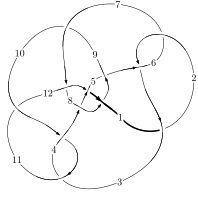
\includegraphics[width=112pt]{../../../GIT/diagram.site/Diagrams/png/1275_12a_0474.png}\\
\ \ \ A knot diagram\footnotemark}&
\allowdisplaybreaks
\textbf{Linearized knot diagam} \\
\cline{2-2}
 &
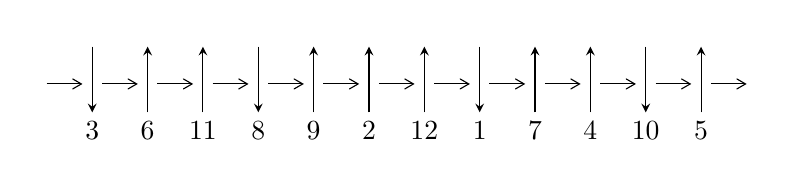
\begin{tikzpicture}[x=20pt, y=17pt]
	% nodes
	\node (C0) at (0, 0) {};
	\node (C1) at (1, 0) {};
	\node (C1U) at (1, +1) {};
	\node (C1D) at (1, -1) {3};

	\node (C2) at (2, 0) {};
	\node (C2U) at (2, +1) {};
	\node (C2D) at (2, -1) {6};

	\node (C3) at (3, 0) {};
	\node (C3U) at (3, +1) {};
	\node (C3D) at (3, -1) {11};

	\node (C4) at (4, 0) {};
	\node (C4U) at (4, +1) {};
	\node (C4D) at (4, -1) {8};

	\node (C5) at (5, 0) {};
	\node (C5U) at (5, +1) {};
	\node (C5D) at (5, -1) {9};

	\node (C6) at (6, 0) {};
	\node (C6U) at (6, +1) {};
	\node (C6D) at (6, -1) {2};

	\node (C7) at (7, 0) {};
	\node (C7U) at (7, +1) {};
	\node (C7D) at (7, -1) {12};

	\node (C8) at (8, 0) {};
	\node (C8U) at (8, +1) {};
	\node (C8D) at (8, -1) {1};

	\node (C9) at (9, 0) {};
	\node (C9U) at (9, +1) {};
	\node (C9D) at (9, -1) {7};

	\node (C10) at (10, 0) {};
	\node (C10U) at (10, +1) {};
	\node (C10D) at (10, -1) {4};

	\node (C11) at (11, 0) {};
	\node (C11U) at (11, +1) {};
	\node (C11D) at (11, -1) {10};

	\node (C12) at (12, 0) {};
	\node (C12U) at (12, +1) {};
	\node (C12D) at (12, -1) {5};
	\node (C13) at (13, 0) {};

	% arrows
	\draw[->,>={angle 60}]
	(C0) edge (C1) (C1) edge (C2) (C2) edge (C3) (C3) edge (C4) (C4) edge (C5) (C5) edge (C6) (C6) edge (C7) (C7) edge (C8) (C8) edge (C9) (C9) edge (C10) (C10) edge (C11) (C11) edge (C12) (C12) edge (C13) ;	\draw[->,>=stealth]
	(C1U) edge (C1D) (C2D) edge (C2U) (C3D) edge (C3U) (C4U) edge (C4D) (C5D) edge (C5U) (C6D) edge (C6U) (C7D) edge (C7U) (C8U) edge (C8D) (C9D) edge (C9U) (C10D) edge (C10U) (C11U) edge (C11D) (C12D) edge (C12U) ;
	\end{tikzpicture} \\
\hhline{~~} \\& 
\textbf{Solving Sequence} \\ \cline{2-2} 
 &
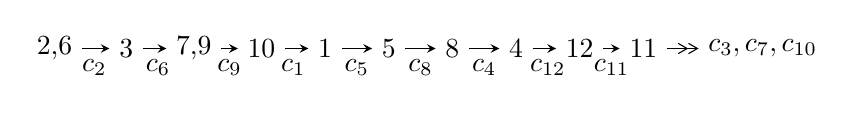
\begin{tikzpicture}[x=23pt, y=7pt]
	% node
	\node (A0) at (-1/8, 0) {2,6};
	\node (A1) at (1, 0) {3};
	\node (A2) at (33/16, 0) {7,9};
	\node (A3) at (25/8, 0) {10};
	\node (A4) at (33/8, 0) {1};
	\node (A5) at (41/8, 0) {5};
	\node (A6) at (49/8, 0) {8};
	\node (A7) at (57/8, 0) {4};
	\node (A8) at (65/8, 0) {12};
	\node (A9) at (73/8, 0) {11};
	\node (C1) at (1/2, -1) {$c_{2}$};
	\node (C2) at (3/2, -1) {$c_{6}$};
	\node (C3) at (21/8, -1) {$c_{9}$};
	\node (C4) at (29/8, -1) {$c_{1}$};
	\node (C5) at (37/8, -1) {$c_{5}$};
	\node (C6) at (45/8, -1) {$c_{8}$};
	\node (C7) at (53/8, -1) {$c_{4}$};
	\node (C8) at (61/8, -1) {$c_{12}$};
	\node (C9) at (69/8, -1) {$c_{11}$};
	\node (A10) at (11, 0) {$c_{3},c_{7},c_{10}$};

	% edge
	\draw[->,>=stealth]	
	(A0) edge (A1) (A1) edge (A2) (A2) edge (A3) (A3) edge (A4) (A4) edge (A5) (A5) edge (A6) (A6) edge (A7) (A7) edge (A8) (A8) edge (A9) ;
	\draw[->>,>={angle 60}]	
	(A9) edge (A10);
\end{tikzpicture} \\ 

\end{tabular} \\

\footnotetext{
The image of knot diagram is generated by the software ``\textbf{Draw programme}" developed by Andrew Bartholomew(\url{http://www.layer8.co.uk/maths/draw/index.htm\#Running-draw}), where we modified some parts for our purpose(\url{https://github.com/CATsTAILs/LinksPainter}).
}\phantom \\ \newline 
\centering \textbf{Ideals for irreducible components\footnotemark of $X_{\text{par}}$} 
 
\begin{align*}
I^u_{1}&=\langle 
1055648117 u^{31}+1559328616 u^{30}+\cdots+2272266299 b+2175618217,\\
\phantom{I^u_{1}}&\phantom{= \langle  }1820724774 u^{31}-1996711433 u^{30}+\cdots+2272266299 a-4457918006,\;u^{32}- u^{31}+\cdots-2 u+1\rangle \\
I^u_{2}&=\langle 
-7.24825\times10^{482} u^{157}-5.26354\times10^{483} u^{156}+\cdots+2.15540\times10^{482} b-2.31148\times10^{486},\\
\phantom{I^u_{2}}&\phantom{= \langle  }-2.62230\times10^{485} u^{157}+3.31275\times10^{486} u^{156}+\cdots+9.03111\times10^{484} a+1.77163\times10^{489},\\
\phantom{I^u_{2}}&\phantom{= \langle  }u^{158}+36 u^{156}+\cdots+795 u+419\rangle \\
I^u_{3}&=\langle 
- u^2+b+u+1,\;a+1,\;u^5+u^3+u^2+u+1\rangle \\
I^u_{4}&=\langle 
-1984676 u^{37}+1585526 u^{36}+\cdots+78131 b+933931,\;u^{37}+12 u^{35}+\cdots+a+1,\\
\phantom{I^u_{4}}&\phantom{= \langle  }u^{38}- u^{37}+\cdots+u+1\rangle \\
I^u_{5}&=\langle 
u^3+u^2+b-1,\;u^3+a,\;u^4+u^3+u^2+u+1\rangle \\
\\
\end{align*}
\raggedright * 5 irreducible components of $\dim_{\mathbb{C}}=0$, with total 237 representations.\\
\footnotetext{All coefficients of polynomials are rational numbers. But the coefficients are sometimes approximated in decimal forms when there is not enough margin.}
\newpage
\renewcommand{\arraystretch}{1}
\centering \section*{I. $I^u_{1}= \langle 1.06\times10^{9} u^{31}+1.56\times10^{9} u^{30}+\cdots+2.27\times10^{9} b+2.18\times10^{9},\;1.82\times10^{9} u^{31}-2.00\times10^{9} u^{30}+\cdots+2.27\times10^{9} a-4.46\times10^{9},\;u^{32}- u^{31}+\cdots-2 u+1 \rangle$}
\flushleft \textbf{(i) Arc colorings}\\
\begin{tabular}{m{7pt} m{180pt} m{7pt} m{180pt} }
\flushright $a_{2}=$&$\begin{pmatrix}1\\0\end{pmatrix}$ \\
\flushright $a_{6}=$&$\begin{pmatrix}0\\u\end{pmatrix}$ \\
\flushright $a_{3}=$&$\begin{pmatrix}1\\- u^2\end{pmatrix}$ \\
\flushright $a_{7}=$&$\begin{pmatrix}u\\u\end{pmatrix}$ \\
\flushright $a_{9}=$&$\begin{pmatrix}-0.801281 u^{31}+0.878731 u^{30}+\cdots-4.37539 u+1.96188\\-0.464579 u^{31}-0.686244 u^{30}+\cdots+2.44777 u-0.957466\end{pmatrix}$ \\
\flushright $a_{10}=$&$\begin{pmatrix}-0.803867 u^{31}+1.07467 u^{30}+\cdots-7.16864 u+3.19015\\-0.467165 u^{31}-0.490301 u^{30}+\cdots-0.345481 u+0.270807\end{pmatrix}$ \\
\flushright $a_{1}=$&$\begin{pmatrix}u^2+1\\- u^4\end{pmatrix}$ \\
\flushright $a_{5}=$&$\begin{pmatrix}0.253688 u^{31}-1.40072 u^{30}+\cdots+6.07370 u-3.05988\\-0.382000 u^{31}-0.403712 u^{30}+\cdots+0.804118 u-0.994004\end{pmatrix}$ \\
\flushright $a_{8}=$&$\begin{pmatrix}-0.773816 u^{31}+0.992632 u^{30}+\cdots-4.85623 u+2.88686\\-0.520128 u^{31}-0.408087 u^{30}+\cdots+1.21747 u-0.173024\end{pmatrix}$ \\
\flushright $a_{4}=$&$\begin{pmatrix}-0.393606 u^{31}+0.511780 u^{30}+\cdots+0.952466 u-0.0779587\\-0.664413 u^{31}+0.315422 u^{30}+\cdots-0.629955 u+0.118174\end{pmatrix}$ \\
\flushright $a_{12}=$&$\begin{pmatrix}-0.454876 u^{31}+1.01874 u^{30}+\cdots-4.95799 u+2.52574\\0.346405 u^{31}+0.140005 u^{30}+\cdots-0.582597 u+0.563860\end{pmatrix}$ \\
\flushright $a_{11}=$&$\begin{pmatrix}-0.922041 u^{31}+0.528435 u^{30}+\cdots-6.30347 u+2.79655\\-0.118174 u^{31}-0.546239 u^{30}+\cdots+0.865171 u-0.393606\end{pmatrix}$\\&\end{tabular}
\flushleft \textbf{(ii) Obstruction class $= -1$}\\~\\
\flushleft \textbf{(iii) Cusp Shapes $= -\frac{3072844380}{2272266299} u^{31}-\frac{8096501151}{2272266299} u^{30}+\cdots+\frac{41644937217}{2272266299} u-\frac{3810236961}{2272266299}$}\\~\\
\newpage\renewcommand{\arraystretch}{1}
\flushleft \textbf{(iv) u-Polynomials at the component}\newline \\
\begin{tabular}{m{50pt}|m{274pt}}
Crossings & \hspace{64pt}u-Polynomials at each crossing \\
\hline $$\begin{aligned}c_{1},c_{11}\end{aligned}$$&$\begin{aligned}
&u^{32}+15 u^{31}+\cdots+6 u+1
\end{aligned}$\\
\hline $$\begin{aligned}c_{2},c_{3},c_{6}\\c_{10}\end{aligned}$$&$\begin{aligned}
&u^{32}- u^{31}+\cdots-2 u+1
\end{aligned}$\\
\hline $$\begin{aligned}c_{4},c_{8}\end{aligned}$$&$\begin{aligned}
&u^{32}+u^{31}+\cdots-9 u^2+1
\end{aligned}$\\
\hline $$\begin{aligned}c_{5},c_{7}\end{aligned}$$&$\begin{aligned}
&u^{32}+u^{31}+\cdots-4 u-1
\end{aligned}$\\
\hline $$\begin{aligned}c_{9}\end{aligned}$$&$\begin{aligned}
&u^{32}+12 u^{31}+\cdots-368 u-320
\end{aligned}$\\
\hline $$\begin{aligned}c_{12}\end{aligned}$$&$\begin{aligned}
&u^{32}-19 u^{31}+\cdots+76 u-8
\end{aligned}$\\
\hline
\end{tabular}\\~\\
\newpage\renewcommand{\arraystretch}{1}
\flushleft \textbf{(v) Riley Polynomials at the component}\newline \\
\begin{tabular}{m{50pt}|m{274pt}}
Crossings & \hspace{64pt}Riley Polynomials at each crossing \\
\hline $$\begin{aligned}c_{1},c_{11}\end{aligned}$$&$\begin{aligned}
&y^{32}+3 y^{31}+\cdots+6 y+1
\end{aligned}$\\
\hline $$\begin{aligned}c_{2},c_{3},c_{6}\\c_{10}\end{aligned}$$&$\begin{aligned}
&y^{32}+15 y^{31}+\cdots+6 y+1
\end{aligned}$\\
\hline $$\begin{aligned}c_{4},c_{8}\end{aligned}$$&$\begin{aligned}
&y^{32}-13 y^{31}+\cdots-18 y+1
\end{aligned}$\\
\hline $$\begin{aligned}c_{5},c_{7}\end{aligned}$$&$\begin{aligned}
&y^{32}-5 y^{31}+\cdots-10 y+1
\end{aligned}$\\
\hline $$\begin{aligned}c_{9}\end{aligned}$$&$\begin{aligned}
&y^{32}-4 y^{31}+\cdots-1748224 y+102400
\end{aligned}$\\
\hline $$\begin{aligned}c_{12}\end{aligned}$$&$\begin{aligned}
&y^{32}-5 y^{31}+\cdots-784 y+64
\end{aligned}$\\
\hline
\end{tabular}\\~\\
\newpage\flushleft \textbf{(vi) Complex Volumes and Cusp Shapes}
$$\begin{array}{c|c|c}  
\text{Solutions to }I^u_{1}& \I (\text{vol} + \sqrt{-1}CS) & \text{Cusp shape}\\
 \hline 
\begin{aligned}
u &= \phantom{-}0.477757 + 0.915446 I \\
a &= \phantom{-}0.822115 + 0.863569 I \\
b &= \phantom{-}2.29964 - 0.04858 I\end{aligned}
 & -3.03094 + 1.03307 I & \phantom{-}1.81391 - 3.75205 I \\ \hline\begin{aligned}
u &= \phantom{-}0.477757 - 0.915446 I \\
a &= \phantom{-}0.822115 - 0.863569 I \\
b &= \phantom{-}2.29964 + 0.04858 I\end{aligned}
 & -3.03094 - 1.03307 I & \phantom{-}1.81391 + 3.75205 I \\ \hline\begin{aligned}
u &= -0.925303 + 0.470201 I \\
a &= \phantom{-}0.77272 + 1.27966 I \\
b &= -0.0866021 + 0.0749753 I\end{aligned}
 & \phantom{-}5.40111 + 9.30081 I & \phantom{-}8.64815 - 4.34110 I \\ \hline\begin{aligned}
u &= -0.925303 - 0.470201 I \\
a &= \phantom{-}0.77272 - 1.27966 I \\
b &= -0.0866021 - 0.0749753 I\end{aligned}
 & \phantom{-}5.40111 - 9.30081 I & \phantom{-}8.64815 + 4.34110 I \\ \hline\begin{aligned}
u &= \phantom{-}1.06263\phantom{ +0.000000I} \\
a &= -0.505330\phantom{ +0.000000I} \\
b &= \phantom{-}0.475352\phantom{ +0.000000I}\end{aligned}
 & \phantom{-}3.35063\phantom{ +0.000000I} & -29.5350\phantom{ +0.000000I} \\ \hline\begin{aligned}
u &= \phantom{-}0.373274 + 0.995878 I \\
a &= -0.659253 + 0.718345 I \\
b &= -1.82629 + 1.33122 I\end{aligned}
 & -0.05576 + 5.19371 I & \phantom{-}4.42887 - 7.08711 I \\ \hline\begin{aligned}
u &= \phantom{-}0.373274 - 0.995878 I \\
a &= -0.659253 - 0.718345 I \\
b &= -1.82629 - 1.33122 I\end{aligned}
 & -0.05576 - 5.19371 I & \phantom{-}4.42887 + 7.08711 I \\ \hline\begin{aligned}
u &= -0.474535 + 0.969658 I \\
a &= -0.744476 + 0.521874 I \\
b &= -1.200380 - 0.655213 I\end{aligned}
 & -3.34712 - 6.37289 I & -0.19797 + 8.93417 I \\ \hline\begin{aligned}
u &= -0.474535 - 0.969658 I \\
a &= -0.744476 - 0.521874 I \\
b &= -1.200380 + 0.655213 I\end{aligned}
 & -3.34712 + 6.37289 I & -0.19797 - 8.93417 I \\ \hline\begin{aligned}
u &= \phantom{-}0.476166 + 1.040000 I \\
a &= -0.853673 + 0.236108 I \\
b &= -2.72342 - 0.90132 I\end{aligned}
 & -2.54495 + 10.44430 I & \phantom{-}0.7629 - 14.2377 I\\
 \hline 
 \end{array}$$\newpage$$\begin{array}{c|c|c}  
\text{Solutions to }I^u_{1}& \I (\text{vol} + \sqrt{-1}CS) & \text{Cusp shape}\\
 \hline 
\begin{aligned}
u &= \phantom{-}0.476166 - 1.040000 I \\
a &= -0.853673 - 0.236108 I \\
b &= -2.72342 + 0.90132 I\end{aligned}
 & -2.54495 - 10.44430 I & \phantom{-}0.7629 + 14.2377 I \\ \hline\begin{aligned}
u &= -0.196973 + 1.132120 I \\
a &= \phantom{-}0.933768 - 0.180629 I \\
b &= \phantom{-}1.58099 - 0.40135 I\end{aligned}
 & -7.68853 - 3.19636 I & -7.98532 + 3.48642 I \\ \hline\begin{aligned}
u &= -0.196973 - 1.132120 I \\
a &= \phantom{-}0.933768 + 0.180629 I \\
b &= \phantom{-}1.58099 + 0.40135 I\end{aligned}
 & -7.68853 + 3.19636 I & -7.98532 - 3.48642 I \\ \hline\begin{aligned}
u &= \phantom{-}1.042280 + 0.520937 I \\
a &= -0.301819 + 0.612779 I \\
b &= \phantom{-}0.408436 + 0.046950 I\end{aligned}
 & \phantom{-}3.94817 - 0.47576 I & \phantom{-}7.7925 + 21.6997 I \\ \hline\begin{aligned}
u &= \phantom{-}1.042280 - 0.520937 I \\
a &= -0.301819 - 0.612779 I \\
b &= \phantom{-}0.408436 - 0.046950 I\end{aligned}
 & \phantom{-}3.94817 + 0.47576 I & \phantom{-}7.7925 - 21.6997 I \\ \hline\begin{aligned}
u &= \phantom{-}0.130483 + 1.162900 I \\
a &= -0.770437 - 0.770567 I \\
b &= -1.25491 - 1.22831 I\end{aligned}
 & -6.42362 - 4.43426 I & -3.93661 + 3.90816 I \\ \hline\begin{aligned}
u &= \phantom{-}0.130483 - 1.162900 I \\
a &= -0.770437 + 0.770567 I \\
b &= -1.25491 + 1.22831 I\end{aligned}
 & -6.42362 + 4.43426 I & -3.93661 - 3.90816 I \\ \hline\begin{aligned}
u &= -0.466499 + 1.079320 I \\
a &= \phantom{-}0.058442 + 0.427246 I \\
b &= \phantom{-}0.630894 - 0.311585 I\end{aligned}
 & -3.17466 - 6.99170 I & -1.77681 + 6.23178 I \\ \hline\begin{aligned}
u &= -0.466499 - 1.079320 I \\
a &= \phantom{-}0.058442 - 0.427246 I \\
b &= \phantom{-}0.630894 + 0.311585 I\end{aligned}
 & -3.17466 + 6.99170 I & -1.77681 - 6.23178 I \\ \hline\begin{aligned}
u &= -0.427864 + 1.109050 I \\
a &= \phantom{-}0.567795 + 0.877389 I \\
b &= \phantom{-}1.48550 + 0.75181 I\end{aligned}
 & -3.53644 - 7.33288 I & -2.60525 + 8.48950 I\\
 \hline 
 \end{array}$$\newpage$$\begin{array}{c|c|c}  
\text{Solutions to }I^u_{1}& \I (\text{vol} + \sqrt{-1}CS) & \text{Cusp shape}\\
 \hline 
\begin{aligned}
u &= -0.427864 - 1.109050 I \\
a &= \phantom{-}0.567795 - 0.877389 I \\
b &= \phantom{-}1.48550 - 0.75181 I\end{aligned}
 & -3.53644 + 7.33288 I & -2.60525 - 8.48950 I \\ \hline\begin{aligned}
u &= \phantom{-}0.667854 + 1.161150 I \\
a &= \phantom{-}1.177840 - 0.492133 I \\
b &= \phantom{-}2.41595 - 1.10503 I\end{aligned}
 & \phantom{-}1.1241 + 21.0689 I & \phantom{-}3.49932 - 11.71002 I \\ \hline\begin{aligned}
u &= \phantom{-}0.667854 - 1.161150 I \\
a &= \phantom{-}1.177840 + 0.492133 I \\
b &= \phantom{-}2.41595 + 1.10503 I\end{aligned}
 & \phantom{-}1.1241 - 21.0689 I & \phantom{-}3.49932 + 11.71002 I \\ \hline\begin{aligned}
u &= -0.490346 + 0.432416 I \\
a &= \phantom{-}0.130078 - 1.235820 I \\
b &= -0.781587 + 0.581190 I\end{aligned}
 & \phantom{-}0.96043 + 2.38010 I & \phantom{-}7.46276 - 4.21750 I \\ \hline\begin{aligned}
u &= -0.490346 - 0.432416 I \\
a &= \phantom{-}0.130078 + 1.235820 I \\
b &= -0.781587 - 0.581190 I\end{aligned}
 & \phantom{-}0.96043 - 2.38010 I & \phantom{-}7.46276 + 4.21750 I \\ \hline\begin{aligned}
u &= -0.683123 + 1.170780 I \\
a &= -0.884504 - 0.167122 I \\
b &= -1.75324 - 0.73186 I\end{aligned}
 & -0.28660 - 12.80370 I & \phantom{-}1.33394 + 11.29862 I \\ \hline\begin{aligned}
u &= -0.683123 - 1.170780 I \\
a &= -0.884504 + 0.167122 I \\
b &= -1.75324 + 0.73186 I\end{aligned}
 & -0.28660 + 12.80370 I & \phantom{-}1.33394 - 11.29862 I \\ \hline\begin{aligned}
u &= -0.219303 + 0.597960 I \\
a &= -0.46196 - 1.88067 I \\
b &= \phantom{-}0.342049 + 0.528048 I\end{aligned}
 & \phantom{-}2.71565 - 0.83716 I & \phantom{-}2.90542 + 8.40033 I \\ \hline\begin{aligned}
u &= -0.219303 - 0.597960 I \\
a &= -0.46196 + 1.88067 I \\
b &= \phantom{-}0.342049 - 0.528048 I\end{aligned}
 & \phantom{-}2.71565 + 0.83716 I & \phantom{-}2.90542 - 8.40033 I \\ \hline\begin{aligned}
u &= \phantom{-}0.441452 + 0.401358 I \\
a &= \phantom{-}0.722248 + 0.018264 I \\
b &= \phantom{-}0.438511 + 0.462396 I\end{aligned}
 & \phantom{-}0.914598 + 0.783161 I & \phantom{-}7.49019 - 4.89846 I\\
 \hline 
 \end{array}$$\newpage$$\begin{array}{c|c|c}  
\text{Solutions to }I^u_{1}& \I (\text{vol} + \sqrt{-1}CS) & \text{Cusp shape}\\
 \hline 
\begin{aligned}
u &= \phantom{-}0.441452 - 0.401358 I \\
a &= \phantom{-}0.722248 - 0.018264 I \\
b &= \phantom{-}0.438511 - 0.462396 I\end{aligned}
 & \phantom{-}0.914598 - 0.783161 I & \phantom{-}7.49019 + 4.89846 I \\ \hline\begin{aligned}
u &= \phantom{-}0.486729\phantom{ +0.000000I} \\
a &= \phantom{-}2.48756\phantom{ +0.000000I} \\
b &= \phantom{-}0.573576\phantom{ +0.000000I}\end{aligned}
 & \phantom{-}2.02457\phantom{ +0.000000I} & \phantom{-}5.26330\phantom{ +0.000000I}\\
 \hline 
 \end{array}$$\newpage\newpage\renewcommand{\arraystretch}{1}
\centering \section*{II. $I^u_{2}= \langle -7.25\times10^{482} u^{157}-5.26\times10^{483} u^{156}+\cdots+2.16\times10^{482} b-2.31\times10^{486},\;-2.62\times10^{485} u^{157}+3.31\times10^{486} u^{156}+\cdots+9.03\times10^{484} a+1.77\times10^{489},\;u^{158}+36 u^{156}+\cdots+795 u+419 \rangle$}
\flushleft \textbf{(i) Arc colorings}\\
\begin{tabular}{m{7pt} m{180pt} m{7pt} m{180pt} }
\flushright $a_{2}=$&$\begin{pmatrix}1\\0\end{pmatrix}$ \\
\flushright $a_{6}=$&$\begin{pmatrix}0\\u\end{pmatrix}$ \\
\flushright $a_{3}=$&$\begin{pmatrix}1\\- u^2\end{pmatrix}$ \\
\flushright $a_{7}=$&$\begin{pmatrix}u\\u\end{pmatrix}$ \\
\flushright $a_{9}=$&$\begin{pmatrix}2.90363 u^{157}-36.6816 u^{156}+\cdots-56119.5 u-19617.0\\3.36284 u^{157}+24.4203 u^{156}+\cdots+33100.0 u+10724.2\end{pmatrix}$ \\
\flushright $a_{10}=$&$\begin{pmatrix}55.5454 u^{157}-42.2460 u^{156}+\cdots-104888. u-45218.7\\56.0046 u^{157}+18.8559 u^{156}+\cdots-15668.4 u-14877.5\end{pmatrix}$ \\
\flushright $a_{1}=$&$\begin{pmatrix}u^2+1\\- u^4\end{pmatrix}$ \\
\flushright $a_{5}=$&$\begin{pmatrix}38.8314 u^{157}+29.1246 u^{156}+\cdots+12999.9 u-2240.90\\29.3771 u^{157}+52.6291 u^{156}+\cdots+54801.0 u+13658.2\end{pmatrix}$ \\
\flushright $a_{8}=$&$\begin{pmatrix}49.9442 u^{157}-33.1921 u^{156}+\cdots-87278.2 u-38257.9\\35.5733 u^{157}+17.8124 u^{156}+\cdots-1422.57 u-6532.33\end{pmatrix}$ \\
\flushright $a_{4}=$&$\begin{pmatrix}-68.6087 u^{157}+82.8124 u^{156}+\cdots+174212. u+71146.3\\-85.6069 u^{157}-11.5076 u^{156}+\cdots+49001.8 u+31342.5\end{pmatrix}$ \\
\flushright $a_{12}=$&$\begin{pmatrix}-42.8030 u^{157}-6.55761 u^{156}+\cdots+22975.2 u+15153.7\\-29.2559 u^{157}-60.7310 u^{156}+\cdots-66924.7 u-17825.3\end{pmatrix}$ \\
\flushright $a_{11}=$&$\begin{pmatrix}-31.0195 u^{157}-23.1998 u^{156}+\cdots-10016.3 u+1903.58\\-52.5109 u^{157}-75.9427 u^{156}+\cdots-71536.0 u-15388.7\end{pmatrix}$\\&\end{tabular}
\flushleft \textbf{(ii) Obstruction class $= -1$}\\~\\
\flushleft \textbf{(iii) Cusp Shapes $= 82.0341 u^{157}+69.2993 u^{156}+\cdots+39167.4 u-737.807$}\\~\\
\newpage\renewcommand{\arraystretch}{1}
\flushleft \textbf{(iv) u-Polynomials at the component}\newline \\
\begin{tabular}{m{50pt}|m{274pt}}
Crossings & \hspace{64pt}u-Polynomials at each crossing \\
\hline $$\begin{aligned}c_{1},c_{11}\end{aligned}$$&$\begin{aligned}
&u^{158}+72 u^{157}+\cdots+3542053 u+175561
\end{aligned}$\\
\hline $$\begin{aligned}c_{2},c_{3},c_{6}\\c_{10}\end{aligned}$$&$\begin{aligned}
&u^{158}+36 u^{156}+\cdots+795 u+419
\end{aligned}$\\
\hline $$\begin{aligned}c_{4},c_{8}\end{aligned}$$&$\begin{aligned}
&u^{158}+4 u^{157}+\cdots-84 u+305
\end{aligned}$\\
\hline $$\begin{aligned}c_{5},c_{7}\end{aligned}$$&$\begin{aligned}
&u^{158}-7 u^{156}+\cdots-1086387 u+160579
\end{aligned}$\\
\hline $$\begin{aligned}c_{9}\end{aligned}$$&$\begin{aligned}
&(u^{79}-12 u^{78}+\cdots-16031 u+5803)^{2}
\end{aligned}$\\
\hline $$\begin{aligned}c_{12}\end{aligned}$$&$\begin{aligned}
&(u^{79}+7 u^{78}+\cdots- u-1)^{2}
\end{aligned}$\\
\hline
\end{tabular}\\~\\
\newpage\renewcommand{\arraystretch}{1}
\flushleft \textbf{(v) Riley Polynomials at the component}\newline \\
\begin{tabular}{m{50pt}|m{274pt}}
Crossings & \hspace{64pt}Riley Polynomials at each crossing \\
\hline $$\begin{aligned}c_{1},c_{11}\end{aligned}$$&$\begin{aligned}
&y^{158}+40 y^{157}+\cdots-2099160591827 y+30821664721
\end{aligned}$\\
\hline $$\begin{aligned}c_{2},c_{3},c_{6}\\c_{10}\end{aligned}$$&$\begin{aligned}
&y^{158}+72 y^{157}+\cdots+3542053 y+175561
\end{aligned}$\\
\hline $$\begin{aligned}c_{4},c_{8}\end{aligned}$$&$\begin{aligned}
&y^{158}+8 y^{157}+\cdots-7749786 y+93025
\end{aligned}$\\
\hline $$\begin{aligned}c_{5},c_{7}\end{aligned}$$&$\begin{aligned}
&y^{158}-14 y^{157}+\cdots-1110681919919 y+25785615241
\end{aligned}$\\
\hline $$\begin{aligned}c_{9}\end{aligned}$$&$\begin{aligned}
&(y^{79}-22 y^{78}+\cdots+521006249 y-33674809)^{2}
\end{aligned}$\\
\hline $$\begin{aligned}c_{12}\end{aligned}$$&$\begin{aligned}
&(y^{79}- y^{78}+\cdots+3 y-1)^{2}
\end{aligned}$\\
\hline
\end{tabular}\\~\\
\newpage\flushleft \textbf{(vi) Complex Volumes and Cusp Shapes}
$$\begin{array}{c|c|c}  
\text{Solutions to }I^u_{2}& \I (\text{vol} + \sqrt{-1}CS) & \text{Cusp shape}\\
 \hline 
\begin{aligned}
u &= -0.310553 + 0.959553 I \\
a &= -1.30464 - 0.80619 I \\
b &= -2.25826 + 0.33876 I\end{aligned}
 & -2.54106 + 5.73014 I & \phantom{-0.000000 } 0 \\ \hline\begin{aligned}
u &= -0.310553 - 0.959553 I \\
a &= -1.30464 + 0.80619 I \\
b &= -2.25826 - 0.33876 I\end{aligned}
 & -2.54106 - 5.73014 I & \phantom{-0.000000 } 0 \\ \hline\begin{aligned}
u &= -0.434056 + 0.885145 I \\
a &= \phantom{-}2.01832 - 1.29649 I \\
b &= \phantom{-}2.40756 - 0.98414 I\end{aligned}
 & -6.62459 - 1.78219 I & \phantom{-0.000000 } 0 \\ \hline\begin{aligned}
u &= -0.434056 - 0.885145 I \\
a &= \phantom{-}2.01832 + 1.29649 I \\
b &= \phantom{-}2.40756 + 0.98414 I\end{aligned}
 & -6.62459 + 1.78219 I & \phantom{-0.000000 } 0 \\ \hline\begin{aligned}
u &= -0.265458 + 0.979005 I \\
a &= \phantom{-}0.115623 + 0.809267 I \\
b &= \phantom{-}0.465376 + 0.297373 I\end{aligned}
 & -4.16298 + 0.24557 I & \phantom{-0.000000 } 0 \\ \hline\begin{aligned}
u &= -0.265458 - 0.979005 I \\
a &= \phantom{-}0.115623 - 0.809267 I \\
b &= \phantom{-}0.465376 - 0.297373 I\end{aligned}
 & -4.16298 - 0.24557 I & \phantom{-0.000000 } 0 \\ \hline\begin{aligned}
u &= -0.568710 + 0.840944 I \\
a &= -0.312373 - 1.146900 I \\
b &= \phantom{-}0.217198 + 0.226950 I\end{aligned}
 & \phantom{-}4.11004 - 1.48250 I & \phantom{-0.000000 } 0 \\ \hline\begin{aligned}
u &= -0.568710 - 0.840944 I \\
a &= -0.312373 + 1.146900 I \\
b &= \phantom{-}0.217198 - 0.226950 I\end{aligned}
 & \phantom{-}4.11004 + 1.48250 I & \phantom{-0.000000 } 0 \\ \hline\begin{aligned}
u &= -0.091908 + 0.977990 I \\
a &= -0.723067 + 0.656630 I \\
b &= -1.76400 + 1.68289 I\end{aligned}
 & -0.54608 + 4.60609 I & \phantom{-0.000000 } 0 \\ \hline\begin{aligned}
u &= -0.091908 - 0.977990 I \\
a &= -0.723067 - 0.656630 I \\
b &= -1.76400 - 1.68289 I\end{aligned}
 & -0.54608 - 4.60609 I & \phantom{-0.000000 } 0\\
 \hline 
 \end{array}$$\newpage$$\begin{array}{c|c|c}  
\text{Solutions to }I^u_{2}& \I (\text{vol} + \sqrt{-1}CS) & \text{Cusp shape}\\
 \hline 
\begin{aligned}
u &= \phantom{-}0.382591 + 0.899744 I \\
a &= \phantom{-}1.68343 - 0.70032 I \\
b &= \phantom{-}2.18485 + 0.24223 I\end{aligned}
 & \phantom{-}0.049532 - 0.236212 I & \phantom{-0.000000 } 0 \\ \hline\begin{aligned}
u &= \phantom{-}0.382591 - 0.899744 I \\
a &= \phantom{-}1.68343 + 0.70032 I \\
b &= \phantom{-}2.18485 - 0.24223 I\end{aligned}
 & \phantom{-}0.049532 + 0.236212 I & \phantom{-0.000000 } 0 \\ \hline\begin{aligned}
u &= -0.735318 + 0.710316 I \\
a &= -0.380441 - 0.803541 I \\
b &= \phantom{-}0.186008 + 0.707821 I\end{aligned}
 & \phantom{-}5.24621 + 0.61229 I & \phantom{-0.000000 } 0 \\ \hline\begin{aligned}
u &= -0.735318 - 0.710316 I \\
a &= -0.380441 + 0.803541 I \\
b &= \phantom{-}0.186008 - 0.707821 I\end{aligned}
 & \phantom{-}5.24621 - 0.61229 I & \phantom{-0.000000 } 0 \\ \hline\begin{aligned}
u &= \phantom{-}0.918664 + 0.319464 I \\
a &= \phantom{-}0.719427 - 0.742569 I \\
b &= \phantom{-}0.356304 + 0.267336 I\end{aligned}
 & \phantom{-}0.049532 - 0.236212 I & \phantom{-0.000000 } 0 \\ \hline\begin{aligned}
u &= \phantom{-}0.918664 - 0.319464 I \\
a &= \phantom{-}0.719427 + 0.742569 I \\
b &= \phantom{-}0.356304 - 0.267336 I\end{aligned}
 & \phantom{-}0.049532 + 0.236212 I & \phantom{-0.000000 } 0 \\ \hline\begin{aligned}
u &= -0.589770 + 0.841559 I \\
a &= \phantom{-}0.881205 + 0.323399 I \\
b &= \phantom{-}1.91030 + 0.99055 I\end{aligned}
 & \phantom{-}4.09867 - 3.13109 I & \phantom{-0.000000 } 0 \\ \hline\begin{aligned}
u &= -0.589770 - 0.841559 I \\
a &= \phantom{-}0.881205 - 0.323399 I \\
b &= \phantom{-}1.91030 - 0.99055 I\end{aligned}
 & \phantom{-}4.09867 + 3.13109 I & \phantom{-0.000000 } 0 \\ \hline\begin{aligned}
u &= \phantom{-}0.481337 + 0.916294 I \\
a &= -0.773779 + 0.323872 I \\
b &= -1.62808 - 1.38929 I\end{aligned}
 & -3.00491 + 3.72449 I & \phantom{-0.000000 } 0 \\ \hline\begin{aligned}
u &= \phantom{-}0.481337 - 0.916294 I \\
a &= -0.773779 - 0.323872 I \\
b &= -1.62808 + 1.38929 I\end{aligned}
 & -3.00491 - 3.72449 I & \phantom{-0.000000 } 0\\
 \hline 
 \end{array}$$\newpage$$\begin{array}{c|c|c}  
\text{Solutions to }I^u_{2}& \I (\text{vol} + \sqrt{-1}CS) & \text{Cusp shape}\\
 \hline 
\begin{aligned}
u &= \phantom{-}0.795996 + 0.675080 I \\
a &= \phantom{-}0.369650 - 0.699877 I \\
b &= -0.105022 + 0.867379 I\end{aligned}
 & \phantom{-}3.75059 - 5.60386 I & \phantom{-0.000000 } 0 \\ \hline\begin{aligned}
u &= \phantom{-}0.795996 - 0.675080 I \\
a &= \phantom{-}0.369650 + 0.699877 I \\
b &= -0.105022 - 0.867379 I\end{aligned}
 & \phantom{-}3.75059 + 5.60386 I & \phantom{-0.000000 } 0 \\ \hline\begin{aligned}
u &= \phantom{-}0.952560 + 0.428199 I \\
a &= -0.80810 + 1.25137 I \\
b &= \phantom{-}0.0918948 - 0.0588807 I\end{aligned}
 & \phantom{-}3.3684 - 15.1632 I & \phantom{-0.000000 } 0 \\ \hline\begin{aligned}
u &= \phantom{-}0.952560 - 0.428199 I \\
a &= -0.80810 - 1.25137 I \\
b &= \phantom{-}0.0918948 + 0.0588807 I\end{aligned}
 & \phantom{-}3.3684 + 15.1632 I & \phantom{-0.000000 } 0 \\ \hline\begin{aligned}
u &= -0.828714 + 0.636993 I \\
a &= \phantom{-}0.56583 + 1.34399 I \\
b &= -0.100191 + 0.581741 I\end{aligned}
 & \phantom{-}6.17644 + 4.30612 I & \phantom{-0.000000 } 0 \\ \hline\begin{aligned}
u &= -0.828714 - 0.636993 I \\
a &= \phantom{-}0.56583 - 1.34399 I \\
b &= -0.100191 - 0.581741 I\end{aligned}
 & \phantom{-}6.17644 - 4.30612 I & \phantom{-0.000000 } 0 \\ \hline\begin{aligned}
u &= \phantom{-}0.398177 + 0.863793 I \\
a &= \phantom{-}0.409774 - 1.284210 I \\
b &= \phantom{-}0.332705 + 0.390561 I\end{aligned}
 & \phantom{-}0.29819 - 2.09088 I & \phantom{-0.000000 } 0 \\ \hline\begin{aligned}
u &= \phantom{-}0.398177 - 0.863793 I \\
a &= \phantom{-}0.409774 + 1.284210 I \\
b &= \phantom{-}0.332705 - 0.390561 I\end{aligned}
 & \phantom{-}0.29819 + 2.09088 I & \phantom{-0.000000 } 0 \\ \hline\begin{aligned}
u &= \phantom{-}0.561309 + 0.748245 I \\
a &= -1.108600 + 0.318648 I \\
b &= -1.87960 + 0.98263 I\end{aligned}
 & \phantom{-}1.98199 - 2.11208 I & \phantom{-0.000000 } 0 \\ \hline\begin{aligned}
u &= \phantom{-}0.561309 - 0.748245 I \\
a &= -1.108600 - 0.318648 I \\
b &= -1.87960 - 0.98263 I\end{aligned}
 & \phantom{-}1.98199 + 2.11208 I & \phantom{-0.000000 } 0\\
 \hline 
 \end{array}$$\newpage$$\begin{array}{c|c|c}  
\text{Solutions to }I^u_{2}& \I (\text{vol} + \sqrt{-1}CS) & \text{Cusp shape}\\
 \hline 
\begin{aligned}
u &= \phantom{-}0.792422 + 0.720401 I \\
a &= -0.424977 + 1.294580 I \\
b &= \phantom{-}0.152595 + 0.766920 I\end{aligned}
 & \phantom{-}4.86883 + 1.98153 I & \phantom{-0.000000 } 0 \\ \hline\begin{aligned}
u &= \phantom{-}0.792422 - 0.720401 I \\
a &= -0.424977 - 1.294580 I \\
b &= \phantom{-}0.152595 - 0.766920 I\end{aligned}
 & \phantom{-}4.86883 - 1.98153 I & \phantom{-0.000000 } 0 \\ \hline\begin{aligned}
u &= \phantom{-}0.795505 + 0.456402 I \\
a &= -0.79974 + 1.42218 I \\
b &= -0.235471 + 0.214744 I\end{aligned}
 & -1.14863 - 6.63514 I & \phantom{-0.000000 } 0 \\ \hline\begin{aligned}
u &= \phantom{-}0.795505 - 0.456402 I \\
a &= -0.79974 - 1.42218 I \\
b &= -0.235471 - 0.214744 I\end{aligned}
 & -1.14863 + 6.63514 I & \phantom{-0.000000 } 0 \\ \hline\begin{aligned}
u &= \phantom{-}0.557057 + 0.929299 I \\
a &= \phantom{-}0.165136 - 1.250270 I \\
b &= -0.354709 - 0.114513 I\end{aligned}
 & \phantom{-}1.40852 + 6.59786 I & \phantom{-0.000000 } 0 \\ \hline\begin{aligned}
u &= \phantom{-}0.557057 - 0.929299 I \\
a &= \phantom{-}0.165136 + 1.250270 I \\
b &= -0.354709 + 0.114513 I\end{aligned}
 & \phantom{-}1.40852 - 6.59786 I & \phantom{-0.000000 } 0 \\ \hline\begin{aligned}
u &= \phantom{-}0.527880 + 0.947283 I \\
a &= -1.45741 - 1.53177 I \\
b &= -2.25677 - 1.07570 I\end{aligned}
 & \phantom{-}1.00763 + 5.22007 I & \phantom{-0.000000 } 0 \\ \hline\begin{aligned}
u &= \phantom{-}0.527880 - 0.947283 I \\
a &= -1.45741 + 1.53177 I \\
b &= -2.25677 + 1.07570 I\end{aligned}
 & \phantom{-}1.00763 - 5.22007 I & \phantom{-0.000000 } 0 \\ \hline\begin{aligned}
u &= \phantom{-}0.431827 + 0.806322 I \\
a &= -0.063102 - 0.407064 I \\
b &= \phantom{-}1.73474 - 0.17811 I\end{aligned}
 & -2.59007 + 0.08562 I & \phantom{-0.000000 } 0 \\ \hline\begin{aligned}
u &= \phantom{-}0.431827 - 0.806322 I \\
a &= -0.063102 + 0.407064 I \\
b &= \phantom{-}1.73474 + 0.17811 I\end{aligned}
 & -2.59007 - 0.08562 I & \phantom{-0.000000 } 0\\
 \hline 
 \end{array}$$\newpage$$\begin{array}{c|c|c}  
\text{Solutions to }I^u_{2}& \I (\text{vol} + \sqrt{-1}CS) & \text{Cusp shape}\\
 \hline 
\begin{aligned}
u &= \phantom{-}0.432313 + 0.805507 I \\
a &= \phantom{-}1.064280 + 0.561916 I \\
b &= \phantom{-}1.19099 - 0.88066 I\end{aligned}
 & -2.62411 + 2.75813 I & \phantom{-0.000000 } 0 \\ \hline\begin{aligned}
u &= \phantom{-}0.432313 - 0.805507 I \\
a &= \phantom{-}1.064280 - 0.561916 I \\
b &= \phantom{-}1.19099 + 0.88066 I\end{aligned}
 & -2.62411 - 2.75813 I & \phantom{-0.000000 } 0 \\ \hline\begin{aligned}
u &= \phantom{-}0.421077 + 1.001710 I \\
a &= -0.20603 + 1.48403 I \\
b &= -0.68683 + 1.63297 I\end{aligned}
 & -0.40858 + 3.12056 I & \phantom{-0.000000 } 0 \\ \hline\begin{aligned}
u &= \phantom{-}0.421077 - 1.001710 I \\
a &= -0.20603 - 1.48403 I \\
b &= -0.68683 - 1.63297 I\end{aligned}
 & -0.40858 - 3.12056 I & \phantom{-0.000000 } 0 \\ \hline\begin{aligned}
u &= -1.001470 + 0.423311 I \\
a &= \phantom{-}0.456088 + 0.775520 I \\
b &= -0.335205 - 0.008493 I\end{aligned}
 & \phantom{-}2.00890 + 6.73082 I & \phantom{-0.000000 } 0 \\ \hline\begin{aligned}
u &= -1.001470 - 0.423311 I \\
a &= \phantom{-}0.456088 - 0.775520 I \\
b &= -0.335205 + 0.008493 I\end{aligned}
 & \phantom{-}2.00890 - 6.73082 I & \phantom{-0.000000 } 0 \\ \hline\begin{aligned}
u &= \phantom{-}0.171636 + 0.889290 I \\
a &= \phantom{-}0.856525 + 0.617603 I \\
b &= \phantom{-}1.29028 + 1.65011 I\end{aligned}
 & \phantom{-}0.996008 + 0.228208 I & \phantom{-0.000000 } 0 \\ \hline\begin{aligned}
u &= \phantom{-}0.171636 - 0.889290 I \\
a &= \phantom{-}0.856525 - 0.617603 I \\
b &= \phantom{-}1.29028 - 1.65011 I\end{aligned}
 & \phantom{-}0.996008 - 0.228208 I & \phantom{-0.000000 } 0 \\ \hline\begin{aligned}
u &= -0.757754 + 0.491337 I \\
a &= -0.59566 - 1.77542 I \\
b &= \phantom{-}0.238053 + 0.058058 I\end{aligned}
 & \phantom{-}4.45408 + 5.94036 I & \phantom{-0.000000 } 0 \\ \hline\begin{aligned}
u &= -0.757754 - 0.491337 I \\
a &= -0.59566 + 1.77542 I \\
b &= \phantom{-}0.238053 - 0.058058 I\end{aligned}
 & \phantom{-}4.45408 - 5.94036 I & \phantom{-0.000000 } 0\\
 \hline 
 \end{array}$$\newpage$$\begin{array}{c|c|c}  
\text{Solutions to }I^u_{2}& \I (\text{vol} + \sqrt{-1}CS) & \text{Cusp shape}\\
 \hline 
\begin{aligned}
u &= \phantom{-}0.474769 + 1.001460 I \\
a &= -0.103439 + 0.715197 I \\
b &= -0.421852 + 0.439449 I\end{aligned}
 & -0.62943 + 2.99422 I & \phantom{-0.000000 } 0 \\ \hline\begin{aligned}
u &= \phantom{-}0.474769 - 1.001460 I \\
a &= -0.103439 - 0.715197 I \\
b &= -0.421852 - 0.439449 I\end{aligned}
 & -0.62943 - 2.99422 I & \phantom{-0.000000 } 0 \\ \hline\begin{aligned}
u &= -0.395583 + 0.794434 I \\
a &= -0.891930 + 0.915396 I \\
b &= -2.02916 - 0.04997 I\end{aligned}
 & -2.62411 + 2.75813 I & \phantom{-0.000000 } 0 \\ \hline\begin{aligned}
u &= -0.395583 - 0.794434 I \\
a &= -0.891930 - 0.915396 I \\
b &= -2.02916 + 0.04997 I\end{aligned}
 & -2.62411 - 2.75813 I & \phantom{-0.000000 } 0 \\ \hline\begin{aligned}
u &= -0.502570 + 0.996824 I \\
a &= -1.369680 - 0.282057 I \\
b &= -2.10107 - 0.03500 I\end{aligned}
 & -5.64126 - 3.23768 I & \phantom{-0.000000 } 0 \\ \hline\begin{aligned}
u &= -0.502570 - 0.996824 I \\
a &= -1.369680 + 0.282057 I \\
b &= -2.10107 + 0.03500 I\end{aligned}
 & -5.64126 + 3.23768 I & \phantom{-0.000000 } 0 \\ \hline\begin{aligned}
u &= \phantom{-}0.778124 + 0.414904 I \\
a &= \phantom{-}1.47017 - 0.37757 I \\
b &= \phantom{-}0.048902 - 0.227058 I\end{aligned}
 & \phantom{-}4.09867 + 3.13109 I & \phantom{-0.000000 } 0 \\ \hline\begin{aligned}
u &= \phantom{-}0.778124 - 0.414904 I \\
a &= \phantom{-}1.47017 + 0.37757 I \\
b &= \phantom{-}0.048902 + 0.227058 I\end{aligned}
 & \phantom{-}4.09867 - 3.13109 I & \phantom{-0.000000 } 0 \\ \hline\begin{aligned}
u &= -0.298166 + 1.079110 I \\
a &= -0.792936 + 0.759993 I \\
b &= -2.26691 + 0.61890 I\end{aligned}
 & -2.59007 - 0.08562 I & \phantom{-0.000000 } 0 \\ \hline\begin{aligned}
u &= -0.298166 - 1.079110 I \\
a &= -0.792936 - 0.759993 I \\
b &= -2.26691 - 0.61890 I\end{aligned}
 & -2.59007 + 0.08562 I & \phantom{-0.000000 } 0\\
 \hline 
 \end{array}$$\newpage$$\begin{array}{c|c|c}  
\text{Solutions to }I^u_{2}& \I (\text{vol} + \sqrt{-1}CS) & \text{Cusp shape}\\
 \hline 
\begin{aligned}
u &= \phantom{-}0.484094 + 0.734137 I \\
a &= -1.99303 - 1.21164 I \\
b &= -2.04533 - 0.41284 I\end{aligned}
 & \phantom{-}1.72808 - 1.04080 I & \phantom{-0.000000 } 0 \\ \hline\begin{aligned}
u &= \phantom{-}0.484094 - 0.734137 I \\
a &= -1.99303 + 1.21164 I \\
b &= -2.04533 + 0.41284 I\end{aligned}
 & \phantom{-}1.72808 + 1.04080 I & \phantom{-0.000000 } 0 \\ \hline\begin{aligned}
u &= -0.086871 + 1.120720 I \\
a &= -0.761688 + 0.387029 I \\
b &= -1.45240 + 0.20255 I\end{aligned}
 & -3.83157 + 0.71992 I & \phantom{-0.000000 } 0 \\ \hline\begin{aligned}
u &= -0.086871 - 1.120720 I \\
a &= -0.761688 - 0.387029 I \\
b &= -1.45240 - 0.20255 I\end{aligned}
 & -3.83157 - 0.71992 I & \phantom{-0.000000 } 0 \\ \hline\begin{aligned}
u &= \phantom{-}0.692083 + 0.535192 I \\
a &= \phantom{-}0.71604 - 1.93417 I \\
b &= -0.135547 - 0.251225 I\end{aligned}
 & \phantom{-}5.24621 - 0.61229 I & \phantom{-0.000000 } 0 \\ \hline\begin{aligned}
u &= \phantom{-}0.692083 - 0.535192 I \\
a &= \phantom{-}0.71604 + 1.93417 I \\
b &= -0.135547 + 0.251225 I\end{aligned}
 & \phantom{-}5.24621 + 0.61229 I & \phantom{-0.000000 } 0 \\ \hline\begin{aligned}
u &= \phantom{-}0.946963 + 0.614514 I \\
a &= -0.730292 + 0.411435 I \\
b &= \phantom{-}0.140681 + 0.065288 I\end{aligned}
 & \phantom{-}6.17644 + 4.30612 I & \phantom{-0.000000 } 0 \\ \hline\begin{aligned}
u &= \phantom{-}0.946963 - 0.614514 I \\
a &= -0.730292 - 0.411435 I \\
b &= \phantom{-}0.140681 - 0.065288 I\end{aligned}
 & \phantom{-}6.17644 - 4.30612 I & \phantom{-0.000000 } 0 \\ \hline\begin{aligned}
u &= -0.954405 + 0.609131 I \\
a &= -0.553862 - 0.689104 I \\
b &= -0.263916 - 0.139116 I\end{aligned}
 & \phantom{-}1.72808 + 1.04080 I & \phantom{-0.000000 } 0 \\ \hline\begin{aligned}
u &= -0.954405 - 0.609131 I \\
a &= -0.553862 + 0.689104 I \\
b &= -0.263916 + 0.139116 I\end{aligned}
 & \phantom{-}1.72808 - 1.04080 I & \phantom{-0.000000 } 0\\
 \hline 
 \end{array}$$\newpage$$\begin{array}{c|c|c}  
\text{Solutions to }I^u_{2}& \I (\text{vol} + \sqrt{-1}CS) & \text{Cusp shape}\\
 \hline 
\begin{aligned}
u &= \phantom{-}1.016630 + 0.510273 I \\
a &= \phantom{-}0.613493 - 0.706283 I \\
b &= \phantom{-}0.146183 + 0.036293 I\end{aligned}
 & \phantom{-}1.00763 - 5.22007 I & \phantom{-0.000000 } 0 \\ \hline\begin{aligned}
u &= \phantom{-}1.016630 - 0.510273 I \\
a &= \phantom{-}0.613493 + 0.706283 I \\
b &= \phantom{-}0.146183 - 0.036293 I\end{aligned}
 & \phantom{-}1.00763 + 5.22007 I & \phantom{-0.000000 } 0 \\ \hline\begin{aligned}
u &= \phantom{-}0.399897 + 1.066680 I \\
a &= \phantom{-}0.798583 + 0.803025 I \\
b &= \phantom{-}2.47682 + 0.34607 I\end{aligned}
 & -3.00491 - 3.72449 I & \phantom{-0.000000 } 0 \\ \hline\begin{aligned}
u &= \phantom{-}0.399897 - 1.066680 I \\
a &= \phantom{-}0.798583 - 0.803025 I \\
b &= \phantom{-}2.47682 - 0.34607 I\end{aligned}
 & -3.00491 + 3.72449 I & \phantom{-0.000000 } 0 \\ \hline\begin{aligned}
u &= -0.546153 + 1.001830 I \\
a &= \phantom{-}1.16381 - 1.42348 I \\
b &= \phantom{-}2.12433 - 1.06698 I\end{aligned}
 & -0.99488 - 11.48250 I & \phantom{-0.000000 } 0 \\ \hline\begin{aligned}
u &= -0.546153 - 1.001830 I \\
a &= \phantom{-}1.16381 + 1.42348 I \\
b &= \phantom{-}2.12433 + 1.06698 I\end{aligned}
 & -0.99488 + 11.48250 I & \phantom{-0.000000 } 0 \\ \hline\begin{aligned}
u &= \phantom{-}0.688376 + 0.501519 I \\
a &= \phantom{-}0.676559 - 0.556792 I \\
b &= \phantom{-}0.265065 + 0.560795 I\end{aligned}
 & \phantom{-}0.996008 + 0.228208 I & \phantom{-0.000000 } 0 \\ \hline\begin{aligned}
u &= \phantom{-}0.688376 - 0.501519 I \\
a &= \phantom{-}0.676559 + 0.556792 I \\
b &= \phantom{-}0.265065 - 0.560795 I\end{aligned}
 & \phantom{-}0.996008 - 0.228208 I & \phantom{-0.000000 } 0 \\ \hline\begin{aligned}
u &= -0.341377 + 1.101100 I \\
a &= -0.508755 + 0.675606 I \\
b &= -1.009930 + 0.460172 I\end{aligned}
 & -4.16298 - 0.24557 I & \phantom{-0.000000 } 0 \\ \hline\begin{aligned}
u &= -0.341377 - 1.101100 I \\
a &= -0.508755 - 0.675606 I \\
b &= -1.009930 - 0.460172 I\end{aligned}
 & -4.16298 + 0.24557 I & \phantom{-0.000000 } 0\\
 \hline 
 \end{array}$$\newpage$$\begin{array}{c|c|c}  
\text{Solutions to }I^u_{2}& \I (\text{vol} + \sqrt{-1}CS) & \text{Cusp shape}\\
 \hline 
\begin{aligned}
u &= -0.586174 + 0.997243 I \\
a &= \phantom{-}0.850903 + 0.360043 I \\
b &= \phantom{-}1.80384 - 0.34155 I\end{aligned}
 & -0.46550 - 7.02513 I & \phantom{-0.000000 } 0 \\ \hline\begin{aligned}
u &= -0.586174 - 0.997243 I \\
a &= \phantom{-}0.850903 - 0.360043 I \\
b &= \phantom{-}1.80384 + 0.34155 I\end{aligned}
 & -0.46550 + 7.02513 I & \phantom{-0.000000 } 0 \\ \hline\begin{aligned}
u &= -0.659887 + 0.965771 I \\
a &= \phantom{-}0.620572 + 0.228337 I \\
b &= \phantom{-}2.05133 + 0.83766 I\end{aligned}
 & \phantom{-}4.45408 - 5.94036 I & \phantom{-0.000000 } 0 \\ \hline\begin{aligned}
u &= -0.659887 - 0.965771 I \\
a &= \phantom{-}0.620572 - 0.228337 I \\
b &= \phantom{-}2.05133 - 0.83766 I\end{aligned}
 & \phantom{-}4.45408 + 5.94036 I & \phantom{-0.000000 } 0 \\ \hline\begin{aligned}
u &= \phantom{-}0.567850 + 1.025580 I \\
a &= -0.487372 + 0.413230 I \\
b &= -1.69268 + 0.63123 I\end{aligned}
 & -0.54608 + 4.60609 I & \phantom{-0.000000 } 0 \\ \hline\begin{aligned}
u &= \phantom{-}0.567850 - 1.025580 I \\
a &= -0.487372 - 0.413230 I \\
b &= -1.69268 - 0.63123 I\end{aligned}
 & -0.54608 - 4.60609 I & \phantom{-0.000000 } 0 \\ \hline\begin{aligned}
u &= -0.942383 + 0.698077 I \\
a &= \phantom{-}0.759295 + 0.419727 I \\
b &= \phantom{-}0.004151 + 0.164350 I\end{aligned}
 & \phantom{-}5.00194 - 9.97884 I & \phantom{-0.000000 } 0 \\ \hline\begin{aligned}
u &= -0.942383 - 0.698077 I \\
a &= \phantom{-}0.759295 - 0.419727 I \\
b &= \phantom{-}0.004151 - 0.164350 I\end{aligned}
 & \phantom{-}5.00194 + 9.97884 I & \phantom{-0.000000 } 0 \\ \hline\begin{aligned}
u &= \phantom{-}0.687123 + 0.953819 I \\
a &= \phantom{-}1.43518 - 0.36327 I \\
b &= \phantom{-}1.78713 - 0.72200 I\end{aligned}
 & \phantom{-}4.14017 + 3.57693 I & \phantom{-0.000000 } 0 \\ \hline\begin{aligned}
u &= \phantom{-}0.687123 - 0.953819 I \\
a &= \phantom{-}1.43518 + 0.36327 I \\
b &= \phantom{-}1.78713 + 0.72200 I\end{aligned}
 & \phantom{-}4.14017 - 3.57693 I & \phantom{-0.000000 } 0\\
 \hline 
 \end{array}$$\newpage$$\begin{array}{c|c|c}  
\text{Solutions to }I^u_{2}& \I (\text{vol} + \sqrt{-1}CS) & \text{Cusp shape}\\
 \hline 
\begin{aligned}
u &= -0.420682 + 1.101670 I \\
a &= -0.277978 + 0.022640 I \\
b &= -0.692295 - 1.062360 I\end{aligned}
 & -3.56315\phantom{ +0.000000I} & \phantom{-0.000000 } 0 \\ \hline\begin{aligned}
u &= -0.420682 - 1.101670 I \\
a &= -0.277978 - 0.022640 I \\
b &= -0.692295 + 1.062360 I\end{aligned}
 & -3.56315\phantom{ +0.000000I} & \phantom{-0.000000 } 0 \\ \hline\begin{aligned}
u &= -0.772390 + 0.270072 I \\
a &= -1.65475 - 0.34539 I \\
b &= \phantom{-}0.161056 - 0.145472 I\end{aligned}
 & \phantom{-}4.11004 + 1.48250 I & \phantom{-0.000000 } 0 \\ \hline\begin{aligned}
u &= -0.772390 - 0.270072 I \\
a &= -1.65475 + 0.34539 I \\
b &= \phantom{-}0.161056 + 0.145472 I\end{aligned}
 & \phantom{-}4.11004 - 1.48250 I & \phantom{-0.000000 } 0 \\ \hline\begin{aligned}
u &= -0.800802 + 0.127364 I \\
a &= -1.009110 - 0.405406 I \\
b &= -0.661979 + 0.172911 I\end{aligned}
 & -0.40858 + 3.12056 I & \phantom{-0.000000 } 0 \\ \hline\begin{aligned}
u &= -0.800802 - 0.127364 I \\
a &= -1.009110 + 0.405406 I \\
b &= -0.661979 - 0.172911 I\end{aligned}
 & -0.40858 - 3.12056 I & \phantom{-0.000000 } 0 \\ \hline\begin{aligned}
u &= -0.714810 + 0.959332 I \\
a &= -0.993714 + 0.509602 I \\
b &= -1.48592 + 0.18951 I\end{aligned}
 & -5.02416 - 2.82268 I & \phantom{-0.000000 } 0 \\ \hline\begin{aligned}
u &= -0.714810 - 0.959332 I \\
a &= -0.993714 - 0.509602 I \\
b &= -1.48592 - 0.18951 I\end{aligned}
 & -5.02416 + 2.82268 I & \phantom{-0.000000 } 0 \\ \hline\begin{aligned}
u &= \phantom{-}0.598092 + 1.038180 I \\
a &= -1.61264 + 0.51271 I \\
b &= -2.88134 + 1.16487 I\end{aligned}
 & \phantom{-}3.75059 + 5.60386 I & \phantom{-0.000000 } 0 \\ \hline\begin{aligned}
u &= \phantom{-}0.598092 - 1.038180 I \\
a &= -1.61264 - 0.51271 I \\
b &= -2.88134 - 1.16487 I\end{aligned}
 & \phantom{-}3.75059 - 5.60386 I & \phantom{-0.000000 } 0\\
 \hline 
 \end{array}$$\newpage$$\begin{array}{c|c|c}  
\text{Solutions to }I^u_{2}& \I (\text{vol} + \sqrt{-1}CS) & \text{Cusp shape}\\
 \hline 
\begin{aligned}
u &= \phantom{-}0.270415 + 1.170310 I \\
a &= \phantom{-}0.560037 - 0.177285 I \\
b &= \phantom{-}0.852233 - 1.052720 I\end{aligned}
 & -1.13423 + 4.13535 I & \phantom{-0.000000 } 0 \\ \hline\begin{aligned}
u &= \phantom{-}0.270415 - 1.170310 I \\
a &= \phantom{-}0.560037 + 0.177285 I \\
b &= \phantom{-}0.852233 + 1.052720 I\end{aligned}
 & -1.13423 - 4.13535 I & \phantom{-0.000000 } 0 \\ \hline\begin{aligned}
u &= -0.653525 + 0.451009 I \\
a &= -0.311978 - 1.140630 I \\
b &= -0.568685 + 0.320566 I\end{aligned}
 & \phantom{-}0.97564 + 2.31172 I & \phantom{-0.000000 } 0 \\ \hline\begin{aligned}
u &= -0.653525 - 0.451009 I \\
a &= -0.311978 + 1.140630 I \\
b &= -0.568685 - 0.320566 I\end{aligned}
 & \phantom{-}0.97564 - 2.31172 I & \phantom{-0.000000 } 0 \\ \hline\begin{aligned}
u &= \phantom{-}0.675893 + 1.002900 I \\
a &= -0.556998 + 0.202352 I \\
b &= -2.14046 + 0.75499 I\end{aligned}
 & \phantom{-}2.72713 + 11.14780 I & \phantom{-0.000000 } 0 \\ \hline\begin{aligned}
u &= \phantom{-}0.675893 - 1.002900 I \\
a &= -0.556998 - 0.202352 I \\
b &= -2.14046 - 0.75499 I\end{aligned}
 & \phantom{-}2.72713 - 11.14780 I & \phantom{-0.000000 } 0 \\ \hline\begin{aligned}
u &= -0.548179 + 1.081710 I \\
a &= \phantom{-}0.984157 + 0.311380 I \\
b &= \phantom{-}2.63681 + 0.00137 I\end{aligned}
 & -0.93553 - 6.97306 I & \phantom{-0.000000 } 0 \\ \hline\begin{aligned}
u &= -0.548179 - 1.081710 I \\
a &= \phantom{-}0.984157 - 0.311380 I \\
b &= \phantom{-}2.63681 - 0.00137 I\end{aligned}
 & -0.93553 + 6.97306 I & \phantom{-0.000000 } 0 \\ \hline\begin{aligned}
u &= -0.501446 + 0.586462 I \\
a &= \phantom{-}1.92864 - 1.20508 I \\
b &= \phantom{-}1.62944 - 0.12929 I\end{aligned}
 & \phantom{-}0.26567 + 7.11077 I & \phantom{-0.000000 } 0 \\ \hline\begin{aligned}
u &= -0.501446 - 0.586462 I \\
a &= \phantom{-}1.92864 + 1.20508 I \\
b &= \phantom{-}1.62944 + 0.12929 I\end{aligned}
 & \phantom{-}0.26567 - 7.11077 I & \phantom{-0.000000 } 0\\
 \hline 
 \end{array}$$\newpage$$\begin{array}{c|c|c}  
\text{Solutions to }I^u_{2}& \I (\text{vol} + \sqrt{-1}CS) & \text{Cusp shape}\\
 \hline 
\begin{aligned}
u &= -0.691640 + 1.020570 I \\
a &= -1.37343 - 0.44280 I \\
b &= -1.97075 - 0.90997 I\end{aligned}
 & \phantom{-}5.00194 - 9.97884 I & \phantom{-0.000000 } 0 \\ \hline\begin{aligned}
u &= -0.691640 - 1.020570 I \\
a &= -1.37343 + 0.44280 I \\
b &= -1.97075 + 0.90997 I\end{aligned}
 & \phantom{-}5.00194 + 9.97884 I & \phantom{-0.000000 } 0 \\ \hline\begin{aligned}
u &= -0.613886 + 1.070870 I \\
a &= \phantom{-}1.46384 + 0.33278 I \\
b &= \phantom{-}2.97199 + 0.98520 I\end{aligned}
 & \phantom{-}2.72713 - 11.14780 I & \phantom{-0.000000 } 0 \\ \hline\begin{aligned}
u &= -0.613886 - 1.070870 I \\
a &= \phantom{-}1.46384 - 0.33278 I \\
b &= \phantom{-}2.97199 - 0.98520 I\end{aligned}
 & \phantom{-}2.72713 + 11.14780 I & \phantom{-0.000000 } 0 \\ \hline\begin{aligned}
u &= -0.430079 + 1.161930 I \\
a &= \phantom{-}0.582615 + 0.761725 I \\
b &= \phantom{-}1.45091 + 1.71180 I\end{aligned}
 & \phantom{-}0.29819 - 2.09088 I & \phantom{-0.000000 } 0 \\ \hline\begin{aligned}
u &= -0.430079 - 1.161930 I \\
a &= \phantom{-}0.582615 - 0.761725 I \\
b &= \phantom{-}1.45091 - 1.71180 I\end{aligned}
 & \phantom{-}0.29819 + 2.09088 I & \phantom{-0.000000 } 0 \\ \hline\begin{aligned}
u &= \phantom{-}0.627639 + 1.099090 I \\
a &= \phantom{-}1.253660 - 0.583782 I \\
b &= \phantom{-}2.28599 - 0.89412 I\end{aligned}
 & -3.05898 + 11.99430 I & \phantom{-0.000000 } 0 \\ \hline\begin{aligned}
u &= \phantom{-}0.627639 - 1.099090 I \\
a &= \phantom{-}1.253660 + 0.583782 I \\
b &= \phantom{-}2.28599 + 0.89412 I\end{aligned}
 & -3.05898 - 11.99430 I & \phantom{-0.000000 } 0 \\ \hline\begin{aligned}
u &= \phantom{-}0.242663 + 0.690109 I \\
a &= -0.488133 - 0.373111 I \\
b &= \phantom{-}1.77767 + 1.25045 I\end{aligned}
 & -0.93553 - 6.97306 I & \phantom{-0.000000 } 0 \\ \hline\begin{aligned}
u &= \phantom{-}0.242663 - 0.690109 I \\
a &= -0.488133 + 0.373111 I \\
b &= \phantom{-}1.77767 - 1.25045 I\end{aligned}
 & -0.93553 + 6.97306 I & \phantom{-0.000000 } 0\\
 \hline 
 \end{array}$$\newpage$$\begin{array}{c|c|c}  
\text{Solutions to }I^u_{2}& \I (\text{vol} + \sqrt{-1}CS) & \text{Cusp shape}\\
 \hline 
\begin{aligned}
u &= -0.636713 + 0.358715 I \\
a &= \phantom{-}0.860813 + 0.227248 I \\
b &= -0.525472 - 0.388495 I\end{aligned}
 & -1.13423 - 4.13535 I & \phantom{-0.000000 } 0 \\ \hline\begin{aligned}
u &= -0.636713 - 0.358715 I \\
a &= \phantom{-}0.860813 - 0.227248 I \\
b &= -0.525472 + 0.388495 I\end{aligned}
 & -1.13423 + 4.13535 I & \phantom{-0.000000 } 0 \\ \hline\begin{aligned}
u &= \phantom{-}0.607768 + 1.124670 I \\
a &= -0.479627 + 0.823560 I \\
b &= -0.68480 + 1.53923 I\end{aligned}
 & \phantom{-}1.98199 + 2.11208 I & \phantom{-0.000000 } 0 \\ \hline\begin{aligned}
u &= \phantom{-}0.607768 - 1.124670 I \\
a &= -0.479627 - 0.823560 I \\
b &= -0.68480 - 1.53923 I\end{aligned}
 & \phantom{-}1.98199 - 2.11208 I & \phantom{-0.000000 } 0 \\ \hline\begin{aligned}
u &= -0.712373 + 1.072990 I \\
a &= \phantom{-}0.827627 + 0.421722 I \\
b &= \phantom{-}1.49660 + 0.42575 I\end{aligned}
 & \phantom{-}0.26567 - 7.11077 I & \phantom{-0.000000 } 0 \\ \hline\begin{aligned}
u &= -0.712373 - 1.072990 I \\
a &= \phantom{-}0.827627 - 0.421722 I \\
b &= \phantom{-}1.49660 - 0.42575 I\end{aligned}
 & \phantom{-}0.26567 + 7.11077 I & \phantom{-0.000000 } 0 \\ \hline\begin{aligned}
u &= -0.833205 + 0.982765 I \\
a &= -0.498767 - 0.403098 I \\
b &= -0.739078 - 0.793596 I\end{aligned}
 & \phantom{-}4.14017 + 3.57693 I & \phantom{-0.000000 } 0 \\ \hline\begin{aligned}
u &= -0.833205 - 0.982765 I \\
a &= -0.498767 + 0.403098 I \\
b &= -0.739078 + 0.793596 I\end{aligned}
 & \phantom{-}4.14017 - 3.57693 I & \phantom{-0.000000 } 0 \\ \hline\begin{aligned}
u &= -0.014022 + 1.301380 I \\
a &= \phantom{-}0.574955 - 0.618539 I \\
b &= \phantom{-}1.10680 - 1.39265 I\end{aligned}
 & -1.14863 + 6.63514 I & \phantom{-0.000000 } 0 \\ \hline\begin{aligned}
u &= -0.014022 - 1.301380 I \\
a &= \phantom{-}0.574955 + 0.618539 I \\
b &= \phantom{-}1.10680 + 1.39265 I\end{aligned}
 & -1.14863 - 6.63514 I & \phantom{-0.000000 } 0\\
 \hline 
 \end{array}$$\newpage$$\begin{array}{c|c|c}  
\text{Solutions to }I^u_{2}& \I (\text{vol} + \sqrt{-1}CS) & \text{Cusp shape}\\
 \hline 
\begin{aligned}
u &= \phantom{-}0.599739 + 1.165620 I \\
a &= -0.818084 + 0.510760 I \\
b &= -1.96007 + 0.61164 I\end{aligned}
 & -2.54106 + 5.73014 I & \phantom{-0.000000 } 0 \\ \hline\begin{aligned}
u &= \phantom{-}0.599739 - 1.165620 I \\
a &= -0.818084 - 0.510760 I \\
b &= -1.96007 - 0.61164 I\end{aligned}
 & -2.54106 - 5.73014 I & \phantom{-0.000000 } 0 \\ \hline\begin{aligned}
u &= \phantom{-}0.788182 + 1.048400 I \\
a &= \phantom{-}0.499498 - 0.312198 I \\
b &= \phantom{-}0.882089 - 0.823699 I\end{aligned}
 & \phantom{-}4.86883 + 1.98153 I & \phantom{-0.000000 } 0 \\ \hline\begin{aligned}
u &= \phantom{-}0.788182 - 1.048400 I \\
a &= \phantom{-}0.499498 + 0.312198 I \\
b &= \phantom{-}0.882089 + 0.823699 I\end{aligned}
 & \phantom{-}4.86883 - 1.98153 I & \phantom{-0.000000 } 0 \\ \hline\begin{aligned}
u &= -0.574520 + 1.185810 I \\
a &= \phantom{-}0.527043 + 0.816309 I \\
b &= \phantom{-}0.86995 + 1.78445 I\end{aligned}
 & \phantom{-}1.40852 - 6.59786 I & \phantom{-0.000000 } 0 \\ \hline\begin{aligned}
u &= -0.574520 - 1.185810 I \\
a &= \phantom{-}0.527043 - 0.816309 I \\
b &= \phantom{-}0.86995 - 1.78445 I\end{aligned}
 & \phantom{-}1.40852 + 6.59786 I & \phantom{-0.000000 } 0 \\ \hline\begin{aligned}
u &= -0.674555 + 1.135350 I \\
a &= -1.212950 - 0.494366 I \\
b &= -2.32315 - 1.08402 I\end{aligned}
 & \phantom{-}3.3684 - 15.1632 I & \phantom{-0.000000 } 0 \\ \hline\begin{aligned}
u &= -0.674555 - 1.135350 I \\
a &= -1.212950 + 0.494366 I \\
b &= -2.32315 + 1.08402 I\end{aligned}
 & \phantom{-}3.3684 + 15.1632 I & \phantom{-0.000000 } 0 \\ \hline\begin{aligned}
u &= \phantom{-}0.145727 + 1.320420 I \\
a &= \phantom{-}0.445515 + 0.388411 I \\
b &= \phantom{-}1.093950 + 0.368109 I\end{aligned}
 & -5.64126 + 3.23768 I & \phantom{-0.000000 } 0 \\ \hline\begin{aligned}
u &= \phantom{-}0.145727 - 1.320420 I \\
a &= \phantom{-}0.445515 - 0.388411 I \\
b &= \phantom{-}1.093950 - 0.368109 I\end{aligned}
 & -5.64126 - 3.23768 I & \phantom{-0.000000 } 0\\
 \hline 
 \end{array}$$\newpage$$\begin{array}{c|c|c}  
\text{Solutions to }I^u_{2}& \I (\text{vol} + \sqrt{-1}CS) & \text{Cusp shape}\\
 \hline 
\begin{aligned}
u &= \phantom{-}0.713434 + 1.135240 I \\
a &= \phantom{-}0.832513 - 0.087903 I \\
b &= \phantom{-}1.56300 - 0.61923 I\end{aligned}
 & \phantom{-}2.00890 + 6.73082 I & \phantom{-0.000000 } 0 \\ \hline\begin{aligned}
u &= \phantom{-}0.713434 - 1.135240 I \\
a &= \phantom{-}0.832513 + 0.087903 I \\
b &= \phantom{-}1.56300 + 0.61923 I\end{aligned}
 & \phantom{-}2.00890 - 6.73082 I & \phantom{-0.000000 } 0 \\ \hline\begin{aligned}
u &= \phantom{-}0.072618 + 1.342030 I \\
a &= -0.540918 - 0.690908 I \\
b &= -1.19943 - 1.46350 I\end{aligned}
 & -3.05898 - 11.99430 I & \phantom{-0.000000 } 0 \\ \hline\begin{aligned}
u &= \phantom{-}0.072618 - 1.342030 I \\
a &= -0.540918 + 0.690908 I \\
b &= -1.19943 + 1.46350 I\end{aligned}
 & -3.05898 + 11.99430 I & \phantom{-0.000000 } 0 \\ \hline\begin{aligned}
u &= \phantom{-}0.717837 + 1.150840 I \\
a &= -0.812804 + 0.435766 I \\
b &= -1.63701 + 0.68784 I\end{aligned}
 & -0.99488 + 11.48250 I & \phantom{-0.000000 } 0 \\ \hline\begin{aligned}
u &= \phantom{-}0.717837 - 1.150840 I \\
a &= -0.812804 - 0.435766 I \\
b &= -1.63701 - 0.68784 I\end{aligned}
 & -0.99488 - 11.48250 I & \phantom{-0.000000 } 0 \\ \hline\begin{aligned}
u &= -0.615962 + 0.117735 I \\
a &= -0.350383 - 0.326259 I \\
b &= -0.680784 + 0.340817 I\end{aligned}
 & -0.62943 + 2.99422 I & \phantom{-0.000000 } 0 \\ \hline\begin{aligned}
u &= -0.615962 - 0.117735 I \\
a &= -0.350383 + 0.326259 I \\
b &= -0.680784 - 0.340817 I\end{aligned}
 & -0.62943 - 2.99422 I & \phantom{-0.000000 } 0 \\ \hline\begin{aligned}
u &= -0.506324 + 0.223289 I \\
a &= \phantom{-}0.15038 + 1.71230 I \\
b &= \phantom{-}0.262077 + 0.264360 I\end{aligned}
 & -3.83157 - 0.71992 I & \phantom{-0.000000 } 0 \\ \hline\begin{aligned}
u &= -0.506324 - 0.223289 I \\
a &= \phantom{-}0.15038 - 1.71230 I \\
b &= \phantom{-}0.262077 - 0.264360 I\end{aligned}
 & -3.83157 + 0.71992 I & \phantom{-0.000000 } 0\\
 \hline 
 \end{array}$$\newpage$$\begin{array}{c|c|c}  
\text{Solutions to }I^u_{2}& \I (\text{vol} + \sqrt{-1}CS) & \text{Cusp shape}\\
 \hline 
\begin{aligned}
u &= \phantom{-}0.02696 + 1.51625 I \\
a &= \phantom{-}0.062685 + 0.348097 I \\
b &= \phantom{-}0.195230 + 0.644220 I\end{aligned}
 & -6.62459 - 1.78219 I & \phantom{-0.000000 } 0 \\ \hline\begin{aligned}
u &= \phantom{-}0.02696 - 1.51625 I \\
a &= \phantom{-}0.062685 - 0.348097 I \\
b &= \phantom{-}0.195230 - 0.644220 I\end{aligned}
 & -6.62459 + 1.78219 I & \phantom{-0.000000 } 0 \\ \hline\begin{aligned}
u &= -0.09409 + 1.55208 I \\
a &= \phantom{-}0.076689 - 0.128034 I \\
b &= \phantom{-}0.207284 - 0.560484 I\end{aligned}
 & -5.02416 + 2.82268 I & \phantom{-0.000000 } 0 \\ \hline\begin{aligned}
u &= -0.09409 - 1.55208 I \\
a &= \phantom{-}0.076689 + 0.128034 I \\
b &= \phantom{-}0.207284 + 0.560484 I\end{aligned}
 & -5.02416 - 2.82268 I & \phantom{-0.000000 } 0 \\ \hline\begin{aligned}
u &= -0.097038 + 0.425642 I \\
a &= \phantom{-}1.50211 - 0.54612 I \\
b &= -0.638989 + 1.096140 I\end{aligned}
 & \phantom{-}0.97564 + 2.31172 I & \phantom{-}6.81449 - 4.45056 I \\ \hline\begin{aligned}
u &= -0.097038 - 0.425642 I \\
a &= \phantom{-}1.50211 + 0.54612 I \\
b &= -0.638989 - 1.096140 I\end{aligned}
 & \phantom{-}0.97564 - 2.31172 I & \phantom{-}6.81449 + 4.45056 I \\ \hline\begin{aligned}
u &= \phantom{-}0.360284 + 0.083987 I \\
a &= \phantom{-}1.22698 + 2.75279 I \\
b &= \phantom{-}0.762809 - 0.918146 I\end{aligned}
 & -0.46550 + 7.02513 I & \phantom{-}4.81797 - 8.69305 I \\ \hline\begin{aligned}
u &= \phantom{-}0.360284 - 0.083987 I \\
a &= \phantom{-}1.22698 - 2.75279 I \\
b &= \phantom{-}0.762809 + 0.918146 I\end{aligned}
 & -0.46550 - 7.02513 I & \phantom{-}4.81797 + 8.69305 I\\
 \hline 
 \end{array}$$\newpage\newpage\renewcommand{\arraystretch}{1}
\centering \section*{III. $I^u_{3}= \langle - u^2+b+u+1,\;a+1,\;u^5+u^3+u^2+u+1 \rangle$}
\flushleft \textbf{(i) Arc colorings}\\
\begin{tabular}{m{7pt} m{180pt} m{7pt} m{180pt} }
\flushright $a_{2}=$&$\begin{pmatrix}1\\0\end{pmatrix}$ \\
\flushright $a_{6}=$&$\begin{pmatrix}0\\u\end{pmatrix}$ \\
\flushright $a_{3}=$&$\begin{pmatrix}1\\- u^2\end{pmatrix}$ \\
\flushright $a_{7}=$&$\begin{pmatrix}u\\u\end{pmatrix}$ \\
\flushright $a_{9}=$&$\begin{pmatrix}-1\\u^2- u-1\end{pmatrix}$ \\
\flushright $a_{10}=$&$\begin{pmatrix}u^4- u^3-1\\u^4- u^3+u^2- u-1\end{pmatrix}$ \\
\flushright $a_{1}=$&$\begin{pmatrix}u^2+1\\- u^4\end{pmatrix}$ \\
\flushright $a_{5}=$&$\begin{pmatrix}- u\\u^3- u^2\end{pmatrix}$ \\
\flushright $a_{8}=$&$\begin{pmatrix}- u^3-1\\- u^3- u-1\end{pmatrix}$ \\
\flushright $a_{4}=$&$\begin{pmatrix}u^3- u^2- u+1\\u^4+2 u^3- u^2+u+1\end{pmatrix}$ \\
\flushright $a_{12}=$&$\begin{pmatrix}- u^4- u\\- u^4- u+1\end{pmatrix}$ \\
\flushright $a_{11}=$&$\begin{pmatrix}u^2- u-1\\- u^4+u^3+u^2- u\end{pmatrix}$\\&\end{tabular}
\flushleft \textbf{(ii) Obstruction class $= 1$}\\~\\
\flushleft \textbf{(iii) Cusp Shapes $= 8 u^4-8 u^3+5 u^2- u+4$}\\~\\
\newpage\renewcommand{\arraystretch}{1}
\flushleft \textbf{(iv) u-Polynomials at the component}\newline \\
\begin{tabular}{m{50pt}|m{274pt}}
Crossings & \hspace{64pt}u-Polynomials at each crossing \\
\hline $$\begin{aligned}c_{1}\end{aligned}$$&$\begin{aligned}
&u^5-2 u^4+3 u^3- u^2- u+1
\end{aligned}$\\
\hline $$\begin{aligned}c_{2},c_{5},c_{7}\\c_{10}\end{aligned}$$&$\begin{aligned}
&u^5+u^3+u^2+u+1
\end{aligned}$\\
\hline $$\begin{aligned}c_{3},c_{6}\end{aligned}$$&$\begin{aligned}
&u^5+u^3- u^2+u-1
\end{aligned}$\\
\hline $$\begin{aligned}c_{4},c_{8}\end{aligned}$$&$\begin{aligned}
&u^5-2 u^4+2 u^3-3 u^2+2 u+1
\end{aligned}$\\
\hline $$\begin{aligned}c_{9}\end{aligned}$$&$\begin{aligned}
&u^5- u^4-2 u^3+5 u^2+u-5
\end{aligned}$\\
\hline $$\begin{aligned}c_{11}\end{aligned}$$&$\begin{aligned}
&u^5+2 u^4+3 u^3+u^2- u-1
\end{aligned}$\\
\hline $$\begin{aligned}c_{12}\end{aligned}$$&$\begin{aligned}
&u^5- u^4- u^3+3 u^2-2 u+1
\end{aligned}$\\
\hline
\end{tabular}\\~\\
\newpage\renewcommand{\arraystretch}{1}
\flushleft \textbf{(v) Riley Polynomials at the component}\newline \\
\begin{tabular}{m{50pt}|m{274pt}}
Crossings & \hspace{64pt}Riley Polynomials at each crossing \\
\hline $$\begin{aligned}c_{1},c_{11}\end{aligned}$$&$\begin{aligned}
&y^5+2 y^4+3 y^3-3 y^2+3 y-1
\end{aligned}$\\
\hline $$\begin{aligned}c_{2},c_{3},c_{5}\\c_{6},c_{7},c_{10}\end{aligned}$$&$\begin{aligned}
&y^5+2 y^4+3 y^3+y^2- y-1
\end{aligned}$\\
\hline $$\begin{aligned}c_{4},c_{8}\end{aligned}$$&$\begin{aligned}
&y^5-4 y^3+3 y^2+10 y-1
\end{aligned}$\\
\hline $$\begin{aligned}c_{9}\end{aligned}$$&$\begin{aligned}
&y^5-5 y^4+16 y^3-39 y^2+51 y-25
\end{aligned}$\\
\hline $$\begin{aligned}c_{12}\end{aligned}$$&$\begin{aligned}
&y^5-3 y^4+3 y^3-3 y^2-2 y-1
\end{aligned}$\\
\hline
\end{tabular}\\~\\
\newpage\flushleft \textbf{(vi) Complex Volumes and Cusp Shapes}
$$\begin{array}{c|c|c}  
\text{Solutions to }I^u_{3}& \I (\text{vol} + \sqrt{-1}CS) & \text{Cusp shape}\\
 \hline 
\begin{aligned}
u &= -0.262247 + 0.873157 I \\
a &= -1.00000\phantom{ +0.000000I} \\
b &= -1.43138 - 1.33112 I\end{aligned}
 & -3.23200 - 4.86949 I & -1.68901 + 5.80392 I \\ \hline\begin{aligned}
u &= -0.262247 - 0.873157 I \\
a &= -1.00000\phantom{ +0.000000I} \\
b &= -1.43138 + 1.33112 I\end{aligned}
 & -3.23200 + 4.86949 I & -1.68901 - 5.80392 I \\ \hline\begin{aligned}
u &= -0.800095\phantom{ +0.000000I} \\
a &= -1.00000\phantom{ +0.000000I} \\
b &= \phantom{-}0.440247\phantom{ +0.000000I}\end{aligned}
 & \phantom{-}3.56186\phantom{ +0.000000I} & \phantom{-}15.3770\phantom{ +0.000000I} \\ \hline\begin{aligned}
u &= \phantom{-}0.662294 + 1.032030 I \\
a &= -1.00000\phantom{ +0.000000I} \\
b &= -2.28874 + 0.33498 I\end{aligned}
 & \phantom{-}1.45107 + 11.01950 I & \phantom{-}3.00067 - 9.96957 I \\ \hline\begin{aligned}
u &= \phantom{-}0.662294 - 1.032030 I \\
a &= -1.00000\phantom{ +0.000000I} \\
b &= -2.28874 - 0.33498 I\end{aligned}
 & \phantom{-}1.45107 - 11.01950 I & \phantom{-}3.00067 + 9.96957 I\\
 \hline 
 \end{array}$$\newpage\newpage\renewcommand{\arraystretch}{1}
\centering \section*{IV. $I^u_{4}= \langle -1.98\times10^{6} u^{37}+1.59\times10^{6} u^{36}+\cdots+7.81\times10^{4} b+9.34\times10^{5},\;u^{37}+12 u^{35}+\cdots+a+1,\;u^{38}- u^{37}+\cdots+u+1 \rangle$}
\flushleft \textbf{(i) Arc colorings}\\
\begin{tabular}{m{7pt} m{180pt} m{7pt} m{180pt} }
\flushright $a_{2}=$&$\begin{pmatrix}1\\0\end{pmatrix}$ \\
\flushright $a_{6}=$&$\begin{pmatrix}0\\u\end{pmatrix}$ \\
\flushright $a_{3}=$&$\begin{pmatrix}1\\- u^2\end{pmatrix}$ \\
\flushright $a_{7}=$&$\begin{pmatrix}u\\u\end{pmatrix}$ \\
\flushright $a_{9}=$&$\begin{pmatrix}- u^{37}-12 u^{35}+\cdots-15 u-1\\25.4019 u^{37}-20.2932 u^{36}+\cdots+27.4983 u-11.9534\end{pmatrix}$ \\
\flushright $a_{10}=$&$\begin{pmatrix}-8.90282 u^{37}-8.70708 u^{36}+\cdots-47.5106 u-7.10873\\17.4991 u^{37}-29.0003 u^{36}+\cdots-5.01231 u-18.0621\end{pmatrix}$ \\
\flushright $a_{1}=$&$\begin{pmatrix}u^2+1\\- u^4\end{pmatrix}$ \\
\flushright $a_{5}=$&$\begin{pmatrix}2 u^{37}-6 u^{36}+\cdots+8 u-7\\-20.8689 u^{37}+31.3164 u^{36}+\cdots+15.2184 u+15.7883\end{pmatrix}$ \\
\flushright $a_{8}=$&$\begin{pmatrix}0.0465372 u^{37}-6.68628 u^{36}+\cdots-26.0102 u-8.56096\\17.2296 u^{37}-12.7400 u^{36}+\cdots+15.9072 u-7.09197\end{pmatrix}$ \\
\flushright $a_{4}=$&$\begin{pmatrix}47.5463 u^{37}-43.5185 u^{36}+\cdots+62.2595 u+6.55671\\34.9682 u^{37}-21.6243 u^{36}+\cdots+45.5719 u+8.68607\end{pmatrix}$ \\
\flushright $a_{12}=$&$\begin{pmatrix}-7.11001 u^{37}+34.2559 u^{36}+\cdots+51.6108 u+38.2171\\-25.1721 u^{37}+35.8190 u^{36}+\cdots+1.59311 u+26.1673\end{pmatrix}$ \\
\flushright $a_{11}=$&$\begin{pmatrix}-20.8051 u^{37}+29.9356 u^{36}+\cdots+11.8040 u+29.6783\\0.0692171 u^{37}-28.6170 u^{36}+\cdots-27.9778 u-16.8464\end{pmatrix}$\\&\end{tabular}
\flushleft \textbf{(ii) Obstruction class $= 1$}\\~\\
\flushleft \textbf{(iii) Cusp Shapes $= \frac{684514}{78131} u^{37}-\frac{1377704}{78131} u^{36}+\cdots+\frac{565695}{78131} u-\frac{4124650}{78131}$}\\~\\
\newpage\renewcommand{\arraystretch}{1}
\flushleft \textbf{(iv) u-Polynomials at the component}\newline \\
\begin{tabular}{m{50pt}|m{274pt}}
Crossings & \hspace{64pt}u-Polynomials at each crossing \\
\hline $$\begin{aligned}c_{1}\end{aligned}$$&$\begin{aligned}
&u^{38}-25 u^{37}+\cdots-29 u+1
\end{aligned}$\\
\hline $$\begin{aligned}c_{2},c_{10}\end{aligned}$$&$\begin{aligned}
&u^{38}- u^{37}+\cdots+u+1
\end{aligned}$\\
\hline $$\begin{aligned}c_{3},c_{6}\end{aligned}$$&$\begin{aligned}
&u^{38}+u^{37}+\cdots- u+1
\end{aligned}$\\
\hline $$\begin{aligned}c_{4},c_{8}\end{aligned}$$&$\begin{aligned}
&u^{38}- u^{37}+\cdots+7 u^2+1
\end{aligned}$\\
\hline $$\begin{aligned}c_{5},c_{7}\end{aligned}$$&$\begin{aligned}
&u^{38}-3 u^{37}+\cdots-11 u+1
\end{aligned}$\\
\hline $$\begin{aligned}c_{9}\end{aligned}$$&$\begin{aligned}
&(u^{19}-7 u^{18}+\cdots+3 u-1)^{2}
\end{aligned}$\\
\hline $$\begin{aligned}c_{11}\end{aligned}$$&$\begin{aligned}
&u^{38}+25 u^{37}+\cdots+29 u+1
\end{aligned}$\\
\hline $$\begin{aligned}c_{12}\end{aligned}$$&$\begin{aligned}
&(u^{19}+2 u^{18}+\cdots+u+1)^{2}
\end{aligned}$\\
\hline
\end{tabular}\\~\\
\newpage\renewcommand{\arraystretch}{1}
\flushleft \textbf{(v) Riley Polynomials at the component}\newline \\
\begin{tabular}{m{50pt}|m{274pt}}
Crossings & \hspace{64pt}Riley Polynomials at each crossing \\
\hline $$\begin{aligned}c_{1},c_{11}\end{aligned}$$&$\begin{aligned}
&y^{38}-11 y^{37}+\cdots-67 y+1
\end{aligned}$\\
\hline $$\begin{aligned}c_{2},c_{3},c_{6}\\c_{10}\end{aligned}$$&$\begin{aligned}
&y^{38}+25 y^{37}+\cdots+29 y+1
\end{aligned}$\\
\hline $$\begin{aligned}c_{4},c_{8}\end{aligned}$$&$\begin{aligned}
&y^{38}+y^{37}+\cdots+14 y+1
\end{aligned}$\\
\hline $$\begin{aligned}c_{5},c_{7}\end{aligned}$$&$\begin{aligned}
&y^{38}+15 y^{37}+\cdots-39 y+1
\end{aligned}$\\
\hline $$\begin{aligned}c_{9}\end{aligned}$$&$\begin{aligned}
&(y^{19}+3 y^{18}+\cdots-13 y-1)^{2}
\end{aligned}$\\
\hline $$\begin{aligned}c_{12}\end{aligned}$$&$\begin{aligned}
&(y^{19}+8 y^{18}+\cdots+y-1)^{2}
\end{aligned}$\\
\hline
\end{tabular}\\~\\
\newpage\flushleft \textbf{(vi) Complex Volumes and Cusp Shapes}
$$\begin{array}{c|c|c}  
\text{Solutions to }I^u_{4}& \I (\text{vol} + \sqrt{-1}CS) & \text{Cusp shape}\\
 \hline 
\begin{aligned}
u &= \phantom{-}0.857291 + 0.471939 I \\
a &= \phantom{-}0.489725 - 0.735021 I \\
b &= \phantom{-}0.521340 + 0.336730 I\end{aligned}
 & \phantom{-}0.471614 - 0.794306 I & \phantom{-}3.56373 + 5.07257 I \\ \hline\begin{aligned}
u &= \phantom{-}0.857291 - 0.471939 I \\
a &= \phantom{-}0.489725 + 0.735021 I \\
b &= \phantom{-}0.521340 - 0.336730 I\end{aligned}
 & \phantom{-}0.471614 + 0.794306 I & \phantom{-}3.56373 - 5.07257 I \\ \hline\begin{aligned}
u &= -0.339881 + 0.974319 I \\
a &= -0.674523 + 0.845710 I \\
b &= -1.83508 - 0.10903 I\end{aligned}
 & -3.73840 + 2.35300 I & -3.19315 - 1.59794 I \\ \hline\begin{aligned}
u &= -0.339881 - 0.974319 I \\
a &= -0.674523 - 0.845710 I \\
b &= -1.83508 + 0.10903 I\end{aligned}
 & -3.73840 - 2.35300 I & -3.19315 + 1.59794 I \\ \hline\begin{aligned}
u &= \phantom{-}0.385555 + 0.887397 I \\
a &= \phantom{-}1.98518 + 1.05174 I \\
b &= \phantom{-}2.23280 + 1.00987 I\end{aligned}
 & -6.80652 + 1.60888 I & -11.9912 + 9.5186 I \\ \hline\begin{aligned}
u &= \phantom{-}0.385555 - 0.887397 I \\
a &= \phantom{-}1.98518 - 1.05174 I \\
b &= \phantom{-}2.23280 - 1.00987 I\end{aligned}
 & -6.80652 - 1.60888 I & -11.9912 - 9.5186 I \\ \hline\begin{aligned}
u &= -0.364564 + 0.968354 I \\
a &= -0.708654 + 1.071120 I \\
b &= \phantom{-}0.009391 + 1.118890 I\end{aligned}
 & \phantom{-}0.07884 - 3.73395 I & \phantom{-}5.32221 + 8.03220 I \\ \hline\begin{aligned}
u &= -0.364564 - 0.968354 I \\
a &= -0.708654 - 1.071120 I \\
b &= \phantom{-}0.009391 - 1.118890 I\end{aligned}
 & \phantom{-}0.07884 + 3.73395 I & \phantom{-}5.32221 - 8.03220 I \\ \hline\begin{aligned}
u &= \phantom{-}0.300960 + 0.993122 I \\
a &= \phantom{-}0.542850 + 0.596656 I \\
b &= -0.822378 + 0.266941 I\end{aligned}
 & -1.89294 + 8.64589 I & \phantom{-}2.93385 - 10.21550 I \\ \hline\begin{aligned}
u &= \phantom{-}0.300960 - 0.993122 I \\
a &= \phantom{-}0.542850 - 0.596656 I \\
b &= -0.822378 - 0.266941 I\end{aligned}
 & -1.89294 - 8.64589 I & \phantom{-}2.93385 + 10.21550 I\\
 \hline 
 \end{array}$$\newpage$$\begin{array}{c|c|c}  
\text{Solutions to }I^u_{4}& \I (\text{vol} + \sqrt{-1}CS) & \text{Cusp shape}\\
 \hline 
\begin{aligned}
u &= \phantom{-}0.848401 + 0.610309 I \\
a &= \phantom{-}0.226580 - 0.874994 I \\
b &= -0.201691 + 0.306571 I\end{aligned}
 & \phantom{-}2.75263 - 5.40942 I & \phantom{-}5.53760 + 5.21975 I \\ \hline\begin{aligned}
u &= \phantom{-}0.848401 - 0.610309 I \\
a &= \phantom{-}0.226580 + 0.874994 I \\
b &= -0.201691 - 0.306571 I\end{aligned}
 & \phantom{-}2.75263 + 5.40942 I & \phantom{-}5.53760 - 5.21975 I \\ \hline\begin{aligned}
u &= \phantom{-}0.259484 + 0.918290 I \\
a &= \phantom{-}0.817419 + 0.208348 I \\
b &= \phantom{-}0.381830 - 1.357280 I\end{aligned}
 & -3.73840 + 2.35300 I & -3.19315 - 1.59794 I \\ \hline\begin{aligned}
u &= \phantom{-}0.259484 - 0.918290 I \\
a &= \phantom{-}0.817419 - 0.208348 I \\
b &= \phantom{-}0.381830 + 1.357280 I\end{aligned}
 & -3.73840 - 2.35300 I & -3.19315 + 1.59794 I \\ \hline\begin{aligned}
u &= -0.348783 + 0.861259 I \\
a &= -1.76105 + 0.29227 I \\
b &= -2.49906 + 1.14696 I\end{aligned}
 & \phantom{-}0.471614 + 0.794306 I & \phantom{-}3.56373 - 5.07257 I \\ \hline\begin{aligned}
u &= -0.348783 - 0.861259 I \\
a &= -1.76105 - 0.29227 I \\
b &= -2.49906 - 1.14696 I\end{aligned}
 & \phantom{-}0.471614 - 0.794306 I & \phantom{-}3.56373 + 5.07257 I \\ \hline\begin{aligned}
u &= \phantom{-}0.299592 + 0.869774 I \\
a &= \phantom{-}1.250900 + 0.117358 I \\
b &= \phantom{-}2.79613 + 1.22391 I\end{aligned}
 & -1.44854 - 6.15707 I & \phantom{-}1.62490 + 4.95559 I \\ \hline\begin{aligned}
u &= \phantom{-}0.299592 - 0.869774 I \\
a &= \phantom{-}1.250900 - 0.117358 I \\
b &= \phantom{-}2.79613 - 1.22391 I\end{aligned}
 & -1.44854 + 6.15707 I & \phantom{-}1.62490 - 4.95559 I \\ \hline\begin{aligned}
u &= -0.764063 + 0.399289 I \\
a &= -0.735506 - 0.785314 I \\
b &= -0.783034 + 0.077087 I\end{aligned}
 & \phantom{-}0.07884 + 3.73395 I & \phantom{-}5.32221 - 8.03220 I \\ \hline\begin{aligned}
u &= -0.764063 - 0.399289 I \\
a &= -0.735506 + 0.785314 I \\
b &= -0.783034 - 0.077087 I\end{aligned}
 & \phantom{-}0.07884 - 3.73395 I & \phantom{-}5.32221 + 8.03220 I\\
 \hline 
 \end{array}$$\newpage$$\begin{array}{c|c|c}  
\text{Solutions to }I^u_{4}& \I (\text{vol} + \sqrt{-1}CS) & \text{Cusp shape}\\
 \hline 
\begin{aligned}
u &= \phantom{-}0.694304 + 0.946157 I \\
a &= -1.112440 - 0.529650 I \\
b &= -1.58387 - 0.19054 I\end{aligned}
 & -4.92954 + 2.76340 I & \phantom{-}32.6505 + 12.4930 I \\ \hline\begin{aligned}
u &= \phantom{-}0.694304 - 0.946157 I \\
a &= -1.112440 + 0.529650 I \\
b &= -1.58387 + 0.19054 I\end{aligned}
 & -4.92954 - 2.76340 I & \phantom{-}32.6505 - 12.4930 I \\ \hline\begin{aligned}
u &= -0.640614 + 1.003430 I \\
a &= \phantom{-}1.220570 + 0.008241 I \\
b &= \phantom{-}2.23544 + 0.44108 I\end{aligned}
 & \phantom{-}2.75263 - 5.40942 I & \phantom{-}4.00000 + 5.21975 I \\ \hline\begin{aligned}
u &= -0.640614 - 1.003430 I \\
a &= \phantom{-}1.220570 - 0.008241 I \\
b &= \phantom{-}2.23544 - 0.44108 I\end{aligned}
 & \phantom{-}2.75263 + 5.40942 I & \phantom{-}4.00000 - 5.21975 I \\ \hline\begin{aligned}
u &= -0.468792 + 1.102810 I \\
a &= \phantom{-}0.379086 + 0.747842 I \\
b &= \phantom{-}1.12862 + 1.42597 I\end{aligned}
 & \phantom{-}0.84871 - 3.68252 I & \phantom{-}7.53677 + 3.79983 I \\ \hline\begin{aligned}
u &= -0.468792 - 1.102810 I \\
a &= \phantom{-}0.379086 - 0.747842 I \\
b &= \phantom{-}1.12862 - 1.42597 I\end{aligned}
 & \phantom{-}0.84871 + 3.68252 I & \phantom{-}7.53677 - 3.79983 I \\ \hline\begin{aligned}
u &= -0.561759 + 1.074280 I \\
a &= \phantom{-}0.824401 + 0.557811 I \\
b &= \phantom{-}1.91991 + 0.06261 I\end{aligned}
 & -1.89294 - 8.64589 I & \phantom{-}4.00000 + 10.21550 I \\ \hline\begin{aligned}
u &= -0.561759 - 1.074280 I \\
a &= \phantom{-}0.824401 - 0.557811 I \\
b &= \phantom{-}1.91991 - 0.06261 I\end{aligned}
 & -1.89294 + 8.64589 I & \phantom{-}4.00000 - 10.21550 I \\ \hline\begin{aligned}
u &= \phantom{-}0.602960 + 1.090830 I \\
a &= -0.799404 + 0.340668 I \\
b &= -2.16981 + 0.04109 I\end{aligned}
 & -1.44854 + 6.15707 I & \phantom{-0.000000 } 0 \\ \hline\begin{aligned}
u &= \phantom{-}0.602960 - 1.090830 I \\
a &= -0.799404 - 0.340668 I \\
b &= -2.16981 - 0.04109 I\end{aligned}
 & -1.44854 - 6.15707 I & \phantom{-0.000000 } 0\\
 \hline 
 \end{array}$$\newpage$$\begin{array}{c|c|c}  
\text{Solutions to }I^u_{4}& \I (\text{vol} + \sqrt{-1}CS) & \text{Cusp shape}\\
 \hline 
\begin{aligned}
u &= -0.295711 + 0.495304 I \\
a &= -1.11636 - 1.55763 I \\
b &= \phantom{-}0.226864 + 0.692206 I\end{aligned}
 & \phantom{-}3.00935\phantom{ +0.000000I} & \phantom{-}10.02954 + 0. I\phantom{ +0.000000I} \\ \hline\begin{aligned}
u &= -0.295711 - 0.495304 I \\
a &= -1.11636 + 1.55763 I \\
b &= \phantom{-}0.226864 - 0.692206 I\end{aligned}
 & \phantom{-}3.00935\phantom{ +0.000000I} & \phantom{-}10.02954 + 0. I\phantom{ +0.000000I} \\ \hline\begin{aligned}
u &= \phantom{-}0.01175 + 1.46500 I \\
a &= -0.002432 + 0.226165 I \\
b &= \phantom{-}0.137257 + 0.136757 I\end{aligned}
 & -6.80652 + 1.60888 I & \phantom{-0.000000 } 0 \\ \hline\begin{aligned}
u &= \phantom{-}0.01175 - 1.46500 I \\
a &= -0.002432 - 0.226165 I \\
b &= \phantom{-}0.137257 - 0.136757 I\end{aligned}
 & -6.80652 - 1.60888 I & \phantom{-0.000000 } 0 \\ \hline\begin{aligned}
u &= \phantom{-}0.06718 + 1.55891 I \\
a &= -0.016024 + 0.205169 I \\
b &= \phantom{-}0.100936 + 0.625989 I\end{aligned}
 & -4.92954 - 2.76340 I & \phantom{-0.000000 } 0 \\ \hline\begin{aligned}
u &= \phantom{-}0.06718 - 1.55891 I \\
a &= -0.016024 - 0.205169 I \\
b &= \phantom{-}0.100936 - 0.625989 I\end{aligned}
 & -4.92954 + 2.76340 I & \phantom{-0.000000 } 0 \\ \hline\begin{aligned}
u &= -0.043310 + 0.386385 I \\
a &= -0.31032 - 2.49305 I \\
b &= -1.295590 + 0.462262 I\end{aligned}
 & \phantom{-}0.84871 + 3.68252 I & \phantom{-}7.53677 - 3.79983 I \\ \hline\begin{aligned}
u &= -0.043310 - 0.386385 I \\
a &= -0.31032 + 2.49305 I \\
b &= -1.295590 - 0.462262 I\end{aligned}
 & \phantom{-}0.84871 - 3.68252 I & \phantom{-}7.53677 + 3.79983 I\\
 \hline 
 \end{array}$$\newpage\newpage\renewcommand{\arraystretch}{1}
\centering \section*{V. $I^u_{5}= \langle u^3+u^2+b-1,\;u^3+a,\;u^4+u^3+u^2+u+1 \rangle$}
\flushleft \textbf{(i) Arc colorings}\\
\begin{tabular}{m{7pt} m{180pt} m{7pt} m{180pt} }
\flushright $a_{2}=$&$\begin{pmatrix}1\\0\end{pmatrix}$ \\
\flushright $a_{6}=$&$\begin{pmatrix}0\\u\end{pmatrix}$ \\
\flushright $a_{3}=$&$\begin{pmatrix}1\\- u^2\end{pmatrix}$ \\
\flushright $a_{7}=$&$\begin{pmatrix}u\\u\end{pmatrix}$ \\
\flushright $a_{9}=$&$\begin{pmatrix}- u^3\\- u^3- u^2+1\end{pmatrix}$ \\
\flushright $a_{10}=$&$\begin{pmatrix}2 u^2+u+1\\u^2+u+2\end{pmatrix}$ \\
\flushright $a_{1}=$&$\begin{pmatrix}u^2+1\\u^3+u^2+u+1\end{pmatrix}$ \\
\flushright $a_{5}=$&$\begin{pmatrix}- u^2\\- u^3-2 u^2- u-1\end{pmatrix}$ \\
\flushright $a_{8}=$&$\begin{pmatrix}u^2+u+1\\u+1\end{pmatrix}$ \\
\flushright $a_{4}=$&$\begin{pmatrix}u^3+u^2+2 u+1\\- u^3- u^2+u\end{pmatrix}$ \\
\flushright $a_{12}=$&$\begin{pmatrix}- u^3- u\\- u\end{pmatrix}$ \\
\flushright $a_{11}=$&$\begin{pmatrix}u^2+u+2\\- u^2+1\end{pmatrix}$\\&\end{tabular}
\flushleft \textbf{(ii) Obstruction class $= 1$}\\~\\
\flushleft \textbf{(iii) Cusp Shapes $= 8 u^3+7 u^2+2 u+6$}\\~\\
\newpage\renewcommand{\arraystretch}{1}
\flushleft \textbf{(iv) u-Polynomials at the component}\newline \\
\begin{tabular}{m{50pt}|m{274pt}}
Crossings & \hspace{64pt}u-Polynomials at each crossing \\
\hline $$\begin{aligned}c_{1},c_{3},c_{6}\\c_{12}\end{aligned}$$&$\begin{aligned}
&u^4- u^3+u^2- u+1
\end{aligned}$\\
\hline $$\begin{aligned}c_{2},c_{5},c_{7}\\c_{10},c_{11}\end{aligned}$$&$\begin{aligned}
&u^4+u^3+u^2+u+1
\end{aligned}$\\
\hline $$\begin{aligned}c_{4},c_{8}\end{aligned}$$&$\begin{aligned}
&u^4+3 u^3+4 u^2+2 u+1
\end{aligned}$\\
\hline $$\begin{aligned}c_{9}\end{aligned}$$&$\begin{aligned}
&u^4-5 u+5
\end{aligned}$\\
\hline
\end{tabular}\\~\\
\newpage\renewcommand{\arraystretch}{1}
\flushleft \textbf{(v) Riley Polynomials at the component}\newline \\
\begin{tabular}{m{50pt}|m{274pt}}
Crossings & \hspace{64pt}Riley Polynomials at each crossing \\
\hline $$\begin{aligned}c_{1},c_{2},c_{3}\\c_{5},c_{6},c_{7}\\c_{10},c_{11},c_{12}\end{aligned}$$&$\begin{aligned}
&y^4+y^3+y^2+y+1
\end{aligned}$\\
\hline $$\begin{aligned}c_{4},c_{8}\end{aligned}$$&$\begin{aligned}
&y^4- y^3+6 y^2+4 y+1
\end{aligned}$\\
\hline $$\begin{aligned}c_{9}\end{aligned}$$&$\begin{aligned}
&y^4+10 y^2-25 y+25
\end{aligned}$\\
\hline
\end{tabular}\\~\\
\newpage\flushleft \textbf{(vi) Complex Volumes and Cusp Shapes}
$$\begin{array}{c|c|c}  
\text{Solutions to }I^u_{5}& \I (\text{vol} + \sqrt{-1}CS) & \text{Cusp shape}\\
 \hline 
\begin{aligned}
u &= \phantom{-}0.309017 + 0.951057 I \\
a &= \phantom{-}0.809017 + 0.587785 I \\
b &= \phantom{-}2.61803\phantom{ +0.000000I}\end{aligned}
 & -3.94784\phantom{ +0.000000I} & -5.51722 + 1.31433 I \\ \hline\begin{aligned}
u &= \phantom{-}0.309017 - 0.951057 I \\
a &= \phantom{-}0.809017 - 0.587785 I \\
b &= \phantom{-}2.61803\phantom{ +0.000000I}\end{aligned}
 & -3.94784\phantom{ +0.000000I} & -5.51722 - 1.31433 I \\ \hline\begin{aligned}
u &= -0.809017 + 0.587785 I \\
a &= -0.309017 - 0.951057 I \\
b &= \phantom{-}0.381966\phantom{ +0.000000I}\end{aligned}
 & \phantom{-}3.94784\phantom{ +0.000000I} & \phantom{-}9.01722 + 2.12663 I \\ \hline\begin{aligned}
u &= -0.809017 - 0.587785 I \\
a &= -0.309017 + 0.951057 I \\
b &= \phantom{-}0.381966\phantom{ +0.000000I}\end{aligned}
 & \phantom{-}3.94784\phantom{ +0.000000I} & \phantom{-}9.01722 - 2.12663 I\\
 \hline 
 \end{array}$$\newpage
\newpage\renewcommand{\arraystretch}{1}
\centering \section*{ VI. u-Polynomials}
\begin{tabular}{m{50pt}|m{274pt}}
Crossings & \hspace{64pt}u-Polynomials at each crossing \\
\hline $$\begin{aligned}c_{1}\end{aligned}$$&$\begin{aligned}
&(u^4- u^3+u^2- u+1)(u^5-2 u^4+3 u^3- u^2- u+1)\\
&\cdot(u^{32}+15 u^{31}+\cdots+6 u+1)(u^{38}-25 u^{37}+\cdots-29 u+1)\\
&\cdot(u^{158}+72 u^{157}+\cdots+3542053 u+175561)
\end{aligned}$\\
\hline $$\begin{aligned}c_{2},c_{10}\end{aligned}$$&$\begin{aligned}
&(u^4+u^3+u^2+u+1)(u^5+u^3+u^2+u+1)(u^{32}- u^{31}+\cdots-2 u+1)\\
&\cdot(u^{38}- u^{37}+\cdots+u+1)(u^{158}+36 u^{156}+\cdots+795 u+419)
\end{aligned}$\\
\hline $$\begin{aligned}c_{3},c_{6}\end{aligned}$$&$\begin{aligned}
&(u^4- u^3+u^2- u+1)(u^5+u^3- u^2+u-1)(u^{32}- u^{31}+\cdots-2 u+1)\\
&\cdot(u^{38}+u^{37}+\cdots- u+1)(u^{158}+36 u^{156}+\cdots+795 u+419)
\end{aligned}$\\
\hline $$\begin{aligned}c_{4},c_{8}\end{aligned}$$&$\begin{aligned}
&(u^4+3 u^3+4 u^2+2 u+1)(u^5-2 u^4+2 u^3-3 u^2+2 u+1)\\
&\cdot(u^{32}+u^{31}+\cdots-9 u^2+1)(u^{38}- u^{37}+\cdots+7 u^2+1)\\
&\cdot(u^{158}+4 u^{157}+\cdots-84 u+305)
\end{aligned}$\\
\hline $$\begin{aligned}c_{5},c_{7}\end{aligned}$$&$\begin{aligned}
&(u^4+u^3+u^2+u+1)(u^5+u^3+u^2+u+1)(u^{32}+u^{31}+\cdots-4 u-1)\\
&\cdot(u^{38}-3 u^{37}+\cdots-11 u+1)(u^{158}-7 u^{156}+\cdots-1086387 u+160579)
\end{aligned}$\\
\hline $$\begin{aligned}c_{9}\end{aligned}$$&$\begin{aligned}
&(u^4-5 u+5)(u^5- u^4+\cdots+u-5)(u^{19}-7 u^{18}+\cdots+3 u-1)^{2}\\
&\cdot(u^{32}+12 u^{31}+\cdots-368 u-320)\\
&\cdot(u^{79}-12 u^{78}+\cdots-16031 u+5803)^{2}
\end{aligned}$\\
\hline $$\begin{aligned}c_{11}\end{aligned}$$&$\begin{aligned}
&(u^4+u^3+u^2+u+1)(u^5+2 u^4+3 u^3+u^2- u-1)\\
&\cdot(u^{32}+15 u^{31}+\cdots+6 u+1)(u^{38}+25 u^{37}+\cdots+29 u+1)\\
&\cdot(u^{158}+72 u^{157}+\cdots+3542053 u+175561)
\end{aligned}$\\
\hline $$\begin{aligned}c_{12}\end{aligned}$$&$\begin{aligned}
&(u^4- u^3+u^2- u+1)(u^5- u^4- u^3+3 u^2-2 u+1)\\
&\cdot((u^{19}+2 u^{18}+\cdots+u+1)^{2})(u^{32}-19 u^{31}+\cdots+76 u-8)\\
&\cdot(u^{79}+7 u^{78}+\cdots- u-1)^{2}
\end{aligned}$\\
\hline
\end{tabular}\newpage\renewcommand{\arraystretch}{1}
\centering \section*{ VII. Riley Polynomials}
\begin{tabular}{m{50pt}|m{274pt}}
Crossings & \hspace{64pt}Riley Polynomials at each crossing \\
\hline $$\begin{aligned}c_{1},c_{11}\end{aligned}$$&$\begin{aligned}
&(y^4+y^3+y^2+y+1)(y^5+2 y^4+3 y^3-3 y^2+3 y-1)\\
&\cdot(y^{32}+3 y^{31}+\cdots+6 y+1)(y^{38}-11 y^{37}+\cdots-67 y+1)\\
&\cdot(y^{158}+40 y^{157}+\cdots-2099160591827 y+30821664721)
\end{aligned}$\\
\hline $$\begin{aligned}c_{2},c_{3},c_{6}\\c_{10}\end{aligned}$$&$\begin{aligned}
&(y^4+y^3+y^2+y+1)(y^5+2 y^4+3 y^3+y^2- y-1)\\
&\cdot(y^{32}+15 y^{31}+\cdots+6 y+1)(y^{38}+25 y^{37}+\cdots+29 y+1)\\
&\cdot(y^{158}+72 y^{157}+\cdots+3542053 y+175561)
\end{aligned}$\\
\hline $$\begin{aligned}c_{4},c_{8}\end{aligned}$$&$\begin{aligned}
&(y^4- y^3+6 y^2+4 y+1)(y^5-4 y^3+3 y^2+10 y-1)\\
&\cdot(y^{32}-13 y^{31}+\cdots-18 y+1)(y^{38}+y^{37}+\cdots+14 y+1)\\
&\cdot(y^{158}+8 y^{157}+\cdots-7749786 y+93025)
\end{aligned}$\\
\hline $$\begin{aligned}c_{5},c_{7}\end{aligned}$$&$\begin{aligned}
&(y^4+y^3+y^2+y+1)(y^5+2 y^4+3 y^3+y^2- y-1)\\
&\cdot(y^{32}-5 y^{31}+\cdots-10 y+1)(y^{38}+15 y^{37}+\cdots-39 y+1)\\
&\cdot(y^{158}-14 y^{157}+\cdots-1110681919919 y+25785615241)
\end{aligned}$\\
\hline $$\begin{aligned}c_{9}\end{aligned}$$&$\begin{aligned}
&(y^4+10 y^2-25 y+25)(y^5-5 y^4+16 y^3-39 y^2+51 y-25)\\
&\cdot(y^{19}+3 y^{18}+\cdots-13 y-1)^{2}\\
&\cdot(y^{32}-4 y^{31}+\cdots-1748224 y+102400)\\
&\cdot(y^{79}-22 y^{78}+\cdots+521006249 y-33674809)^{2}
\end{aligned}$\\
\hline $$\begin{aligned}c_{12}\end{aligned}$$&$\begin{aligned}
&(y^4+y^3+y^2+y+1)(y^5-3 y^4+3 y^3-3 y^2-2 y-1)\\
&\cdot((y^{19}+8 y^{18}+\cdots+y-1)^{2})(y^{32}-5 y^{31}+\cdots-784 y+64)\\
&\cdot(y^{79}- y^{78}+\cdots+3 y-1)^{2}
\end{aligned}$\\
\hline
\end{tabular}
\vskip 2pc
\end{document}